%% ArcFS – Journal Version
%% Targeting: Future Generation Computer Systems (Elsevier)
%% NOTE FOR AUTHORS: Before final submission, switch \documentclass to
%% Elsevier's elsarticle class and apply the FGCS author guidelines.
%% Content edits below are template-independent.

\documentclass[journal]{IEEEtran}
\IEEEoverridecommandlockouts

\usepackage{cite}
\usepackage{amsmath,amssymb,amsfonts}
\usepackage{algorithm}
\usepackage{algorithmic}
\usepackage{graphicx}
\usepackage{textcomp}
\usepackage{xcolor}
\usepackage{booktabs}
\usepackage{microtype}
\usepackage{url}
\usepackage{multirow}
\usepackage{listings}
\usepackage{balance}
\usepackage{array}

\lstset{
  basicstyle=\ttfamily\small,
  breaklines=true,
  frame=none,
  xleftmargin=1em
}

\def\BibTeX{{\rm B\kern-.05em{\sc i\kern-.025em b}\kern-.08em
    T\kern-.1667em\lower.7ex\hbox{E}\kern-.125emX}}

\begin{document}

\title{ArcFS: A Content-Addressable FUSE Filesystem\\
with Inline Deduplication, Copy-on-Write Versioning,\\
and Semantic Tag Navigation}

\author{
\IEEEauthorblockN{Anandkumar N S,\;
                  Dhakkshin S R,\;
                  Kishoreadhith V,\;
                  M Raj Ragavender,\;
                  Rithvik K}
\IEEEauthorblockA{\textit{Department of Computer Science and Engineering}\\
\textit{PSG College of Technology, Anna University}\\
Coimbatore, India -- 641\,004\\
\{22z209, 22z215, 22z232, 22z233, 22z253\}@psgtech.ac.in}
\and
\IEEEauthorblockN{Dr.\ Arul Anand N (Faculty Guide)}
\IEEEauthorblockA{\textit{Department of Computer Science and Engineering}\\
\textit{PSG College of Technology}\\
Coimbatore, India -- 641\,004}
}

\maketitle

%% ─────────────────────────────────────────────────────────────────────────────
\begin{abstract}
Traditional filesystems store data by location, which prevents native
deduplication, makes versioning expensive, and confines every file to a
single position in the directory hierarchy. We present ArcFS, a
user-space filesystem implemented in Rust that integrates three storage
optimizations into a single transparent write path:
(i)~content-defined chunking (CDC) via a FastCDC Gear-hash engine with
a 256-entry lookup table, producing chunks between 2\,KB and 64\,KB at
a 4\,KB probabilistic target;
(ii)~SHA-256 content-addressable storage (CAS) with per-chunk Zstandard
level-3 compression, where the hash is computed over uncompressed bytes
before any compression transform; and
(iii)~copy-on-write (CoW) snapshots implemented at the recipe-pointer
level, making snapshot creation O(1) in chunk bytes (no data is
copied) at an O($n_i$) sled cost proportional to live inode count
$n_i$.

A semantic virtual filesystem layer (TagFS) overlays the namespace and
resolves composite tag paths through lazy set-intersection over
dual-structure in-memory maps, allowing files to appear under multiple
tag hierarchies without data duplication.  The write-back page cache is
implemented as a \texttt{HashMap\textless{}u64,(Vec\textless{}u8\textgreater{},bool)\textgreater{}}
bounded at 1,024 entries by an LRU policy maintained through a
companion \texttt{VecDeque\textless{}u64\textgreater{}}, deferring the
computationally expensive CAS pipeline to eviction, \texttt{fsync},
or file release.

ArcFS is evaluated against ext4, Btrfs, and a bindfs FUSE pass-through
baseline across three benchmark classes (responsive, durable, integrity)
and a four-profile disk-usage suite. In the responsive (asynchronous)
class, ArcFS achieves 4,275\,MB/s sequential write throughput, a
9.2$\times$ advantage over ext4, by coalescing writes entirely in
the bounded-memory cache. On storage efficiency, it reduces
identical-file storage by 83.7\%, cuts mixed-workload disk consumption
by 57.6\% relative to ext4, and holds snapshot storage costs within
1.3$\times$ of kernel-native Btrfs CoW. All CRC32c integrity
verifications return zero errors, confirming lossless reconstruction
through the full chunking, compression, and decompression pipeline.
We additionally characterize the system's design trade-offs and
limitations, including the offline nature of garbage collection, the
O(n) LRU-update cost, and the residual metadata growth from snapshot
recipe entries.  ArcFS serves as a concrete foundation for cloud
storage primitives---container image layer caches, build artifact stores,
and scientific data archives---where inline deduplication and semantic
navigation reduce both storage cost and retrieval latency across large,
redundant corpora.
\end{abstract}

\begin{IEEEkeywords}
content-addressable storage, data deduplication, content-defined
chunking, FUSE, copy-on-write, semantic filesystem, garbage collection,
Rust
\end{IEEEkeywords}

%% ─────────────────────────────────────────────────────────────────────────────
\section{Introduction}

Modern storage workloads simultaneously demand storage efficiency,
revision history, and flexible retrieval. Conventional Linux filesystems
address each requirement in isolation. Ext4 overwrites data in place,
supports no deduplication, and delegates versioning entirely to
application-layer tools. Btrfs adds copy-on-write snapshots and optional
transparent compression but lacks cross-file content deduplication
without an offline pass through a tool such as \texttt{duperemove}.
Neither system supports semantic organization beyond the directory tree.

Application-level deduplicators such as Restic~\cite{restic2024} and
BorgBackup~\cite{borgbackup2024} perform content-defined chunking
effectively: both tools split archive content into variable-size
chunks that are hashed and stored in flat content-addressed
repositories, achieving significant space savings for backup
workloads. Their benefits, however, do not extend to the filesystem
layer: the underlying storage still writes every byte verbatim, and
space savings require all applications to opt into the specific backup
agent. Cloud storage systems face the same gap at scale---tenant VMs
writing to shared block storage, build pipelines writing duplicate
artifacts, and scientific workflows producing near-identical output
files all generate redundant data that per-application tools cannot
collectively deduplicate. Building these optimizations into the
filesystem layer removes the coordination burden from individual
applications and makes space savings automatic and transparent across
all writers, regardless of language, framework, or access pattern.

A Filesystem in Userspace (FUSE) implementation offers a practical path
to experimenting with such a design without kernel modifications, but
three engineering challenges arise. First, every VFS call crosses the
kernel/user boundary twice, imposing context-switch latency documented at
up to 83 round trips per file read~\cite{vangoor2017fuse}. Second,
deduplication systems that share chunk payloads across inodes require
careful metadata management to maintain consistency across concurrent
writers~\cite{soules2003metadata}. Third, in-memory hash tables mapping
chunk digests to their CAS addresses grow unboundedly with dataset size
unless the design imposes an explicit eviction policy~\cite{zhu2008dedup}.

ArcFS addresses all three challenges within a single Rust prototype.
A write-back page cache---typed as
\texttt{HashMap\textless{}u64,\;(Vec\textless{}u8\textgreater{},\;bool)\textgreater{}}
and bounded at 1,024 entries by an LRU eviction policy maintained through
a companion \texttt{VecDeque\textless{}u64\textgreater{}}---coalesces
small writes before committing them to the CAS pipeline, reducing the
per-write FUSE round-trip count. The sled embedded database~\cite{sled2024}
provides ACID key-value semantics with a prefixed key schema that encodes
inode-to-recipe mappings as separate relations from chunk payloads,
isolating logical metadata from immutable physical data.  The LRU bound
imposes a hard upper bound on the in-memory footprint regardless of
dataset size.

The contributions of this paper are as follows:
\begin{enumerate}
\item \textbf{Unified pipeline design.} A five-layer storage pipeline---FUSE
  interface, write-back LRU cache, FastCDC chunking engine, SHA-256 CAS
  storage, and sled metadata engine---in which each layer is independently
  testable and adjacent layers communicate through narrow byte-stream or
  hash-set contracts.  We show that these layers can be composed in a
  single user-space daemon without kernel modifications.

\item \textbf{Per-file chunker isolation as a design choice.} The
  decision to instantiate a fresh \texttt{Chunker} per file ingestion
  (rather than sharing rolling hash state across files) is a deliberate
  design choice that prevents cross-file boundary interference at the cost
  of forgoing any cross-file boundary correlation that might improve
  deduplication on structurally similar files (e.g., log rotation).
  We characterize the tradeoff and show that the resulting deduplication
  ratio of 83.7\% on identical-file workloads remains competitive with
  kernel-level reflink.

\item \textbf{Mark-and-sweep GC over a dual-store system.} The two-phase
  offline garbage collector---sled prefix scan for the active hash set,
  followed by a CAS directory walk---is a design choice that avoids
  per-chunk reference counting (which would require atomic increments on
  every dedup hit) in favor of a periodic batch sweep.  We characterize
  the memory cost of the active set ($64\,\mathrm{B} \times$ unique
  referenced chunks) and identify the snapshot-deletion recipe-leak that
  makes the GC conservative in practice.

\item \textbf{TagFS virtual ontology engine.} A semantic navigation layer
  that resolves composite tag paths via lazy set-intersection over dual
  in-memory maps, backed by a persistent sled store, with mount-time
  hydration cost proportional to tagged file count rather than total file
  count.  The control interface accepts live tag mutations via a sentinel
  file without requiring a remount cycle.

\item \textbf{Benchmark methodology separating acceptance-path from
  persistence-path cost.} A three-class benchmark campaign (responsive,
  durable, integrity) plus a four-profile disk-usage suite, showing that
  the 9.2$\times$ write throughput advantage over ext4 is attributable
  entirely to write-back coalescing and collapses to near-parity under
  durable fsync semantics.

\item \textbf{Honest limitation characterization.} A quantified analysis
  of the design's failure modes: the GC concurrent-use safety window,
  the O(n) LRU-update cost at 1,024-inode cache capacity, the
  permanent storage growth from snapshot recipe leaks, the absence of
  on-read hash verification, and the single-threaded FUSE dispatch model.
\end{enumerate}

%% ─────────────────────────────────────────────────────────────────────────────
\section{Background and Motivation}

\subsection{Content-Defined Chunking}

Variable-size content-defined chunking partitions a byte stream into
chunks whose boundaries are determined by the content itself rather than
fixed offsets.  The central virtue of CDC is boundary stability: inserting
or deleting $k$ bytes at position $p$ perturbs at most the two chunks
straddling $p$; all other boundaries remain unchanged, preserving their
SHA-256 hashes and therefore their CAS blobs.  Fixed-size chunking lacks
this property entirely: a single-byte insertion at offset 0 shifts every
downstream boundary by one byte, destroying all hash matches for a file
that is otherwise 99.9\% identical.

The dominant boundary-detection approach uses a rolling hash.  The classic
Rabin fingerprint polynomial hash used by LBFS~\cite{muthitacharoen2001lbfs}
processes one byte per polynomial evaluation.  FastCDC~\cite{xia2016fastcdc}
replaces polynomial arithmetic with a single 256-entry lookup table (the
Gear matrix), reducing boundary evaluation to one table lookup and one
left-shift-and-add per byte while preserving boundary entropy.

\subsection{Content-Addressable Storage}

A content-addressable store (CAS) maps content to a canonical identifier
derived entirely from the content, typically a cryptographic hash.  Two
byte strings with the same hash map to the same identifier; therefore,
storing the second copy requires only a pointer, not additional bytes.
Deduplication is implicit: the store checks for the existence of the
destination path before writing.  Venti~\cite{quinlan2002venti}, the Plan
9 network storage server, pioneered the use of SHA-1 CAS for archival
storage, demonstrating that a flat hash-addressed store is a natural
substrate for deduplication and that immutable blobs enable safe sharing
across divergent revisions.

\subsection{Write-Back Caching in User-Space Filesystems}

FUSE imposes a per-request kernel/user round trip.  For a workload that
issues $n$ write system calls, a naive FUSE implementation triggers $n$
pipeline invocations, each crossing the boundary twice.  Write-back
caching coalesces these: each write updates an in-memory buffer and
returns immediately to the caller; the pipeline runs only at eviction,
\texttt{fsync}, or file close.  The throughput ceiling shifts from
physical-media latency to FUSE IPC bandwidth, which is bounded by the
kernel ring buffer and CPU, not the disk.

%% ─────────────────────────────────────────────────────────────────────────────
\section{Related Work}

\subsection{Semantic and Tag-Based Filesystems}

Gifford et al.~\cite{gifford1991semantic} proposed semantic file systems
in which handler programs automatically derive file attributes from content,
decoupling logical organization from physical location. Bloehdorn and
V\"{o}lkel~\cite{bloehdorn2006tagfs} demonstrated tag-based hierarchical
navigation through explicit metadata annotations at the VFS level, showing
that virtual directory construction from tag intersections is feasible
without modifying application binaries.

ArcFS extends this approach in two ways. First, intersections are computed
lazily at \texttt{readdir} time over dual in-memory maps rather than
materialized on disk, avoiding the write amplification of pre-computing all
tag intersections.  Second, the tag control file (\texttt{.tagfs\_ctl}) at
the filesystem root accepts line-oriented \texttt{set} and \texttt{del}
commands without requiring an unmount cycle, enabling live tag mutation from
any POSIX-compatible process.

\subsection{Content-Defined Chunking and Deduplication}

The Low-Bandwidth Network Filesystem (LBFS)~\cite{muthitacharoen2001lbfs}
introduced content-defined chunking with Rabin fingerprints to suppress
redundant network transfers. Zhu et al.~\cite{zhu2008dedup} demonstrated
that combining CDC with content-addressed storage substantially reduces
backup storage; their Data Domain system processes chunk fingerprints
through an in-memory bloom filter and a similarity index before issuing
disk I/O, bounding memory even for petabyte-scale datasets.

BorgBackup~\cite{borgbackup2024} applies CDC deduplication at the
application layer, chunking archive content into variable-size segments
that are hashed, encrypted, and stored in a flat repository.  Unlike ArcFS,
Borg operates outside the filesystem and requires all clients to use the
same backup agent; space savings are not shared across arbitrary writers.

ArcFS adopts the FastCDC algorithm~\cite{xia2016fastcdc} with a 256-entry
Gear-hash lookup table, which replaces the polynomial arithmetic of Rabin
fingerprinting with a single table lookup per byte, lowering chunking CPU
cost while preserving boundary entropy.  The Gear matrix is built at compile
time via a \texttt{const fn} that chains \texttt{splitmix64}-derived 64-bit
values seeded from a fixed 64-bit constant.

\subsection{Copy-on-Write Filesystems}

Rosenblum and Ousterhout~\cite{rosenblum1992lfs} established the
log-structured filesystem, providing the structural foundation for efficient
CoW semantics. Btrfs and ZFS operationalize this idea for production
workloads, sharing unchanged extents across snapshot subvolumes through
kernel-level reference-counted B-tree nodes.

ArcFS applies the same principle at the recipe level: a snapshot is a
\texttt{SnapshotMetadata} record (name, Unix timestamp, root inode ID)
persisted in sled.  The snapshot's inode tree is materialized by deep-cloning
live inode metadata---assigning new inode IDs while copying recipe
pointers---so snapshot and live namespaces share CAS blobs without copying
them.  Snapshot creation is O(1) in CAS operations (no chunk bytes are
duplicated); the sled-level cost is O($n_i$) where $n_i$ is the number of
live inodes, as each inode's \texttt{ino\_meta:} and \texttt{ino\_recipe:}
records must be cloned.  For a 200\,MB base with $\sim$1{,}000 inodes, this
represents approximately 2{,}000 sled writes plus flush calls, which
completes in milliseconds on modern NVMe storage.

\subsection{Write-Optimized Data Structures and Storage Engines}

BetrFS~\cite{jannen2015betrfs} demonstrates that B\textsuperscript{$\varepsilon$}-trees,
a write-optimized variant of B-trees that buffers updates in internal nodes
and flushes them in large batches, can substantially improve sequential and
random write throughput for filesystem metadata compared to conventional
B-tree layouts.  ArcFS uses sled, a concurrent B-tree engine written in
Rust~\cite{sled2024}, rather than a write-optimized tree, making metadata
write performance proportional to the sled B-tree's update cost plus the
cost of \texttt{flush()}.  Adopting a write-optimized metadata engine is a
natural direction for future work.

WiscKey~\cite{lu2017wisckey} separates B-tree index keys from their
associated values, storing values in a circular log and indexing them by
key in a compact LSM tree. This design substantially reduces write
amplification for large values relative to log-structured merge trees that
co-locate keys and values. ArcFS implicitly separates chunk data (the
CAS blobs on the POSIX filesystem) from chunk identifiers (SHA-256 hex
strings in sled), achieving a similar key-value separation at the
storage-engine boundary. Unlike WiscKey, CAS blobs in ArcFS are immutable
once written; there is no garbage-collection pressure from value overwriting.

\subsection{Distributed and Networked Filesystems}

Ceph~\cite{weil2006ceph} provides a distributed filesystem built on RADOS,
a reliable, autonomous distributed object store. CephFS exposes a
POSIX-compatible interface over RADOS objects, scaling metadata across
multiple MDS daemons using a dynamic subtree partitioning algorithm.
ArcFS occupies the opposite end of the deployment spectrum: a single-node
user-space daemon with no distributed coordination layer.  The CAS storage
directory in ArcFS could in principle be replaced by a distributed
object store (e.g., a RADOS pool or an S3-compatible endpoint), extending
ArcFS into a lightweight distributed deduplication gateway; this is
reserved for future work.

\subsection{User-Space Filesystem Performance}

Vangoor et al.~\cite{vangoor2017fuse} systematically characterized FUSE
overhead and showed that request coalescing can recover a large fraction of
the penalty. Miller et al.~\cite{miller2021bento} demonstrated Rust-based
in-kernel modules that eliminate context-switch cost entirely, approaching
native throughput. ArcFS operates in user space and uses a write-back
cache as its primary mitigation strategy, trading some durability-path
latency for substantial acceptance-path throughput.

\subsection{Applicability to Cloud Storage Workloads}

The design patterns in ArcFS address workloads that arise repeatedly in
cloud infrastructure.  Container image layers are highly redundant
(base images shared across thousands of containers) and benefit directly
from CDC deduplication: each layer's files are chunked on write, and
shared base-layer content produces SHA-256 hash collisions that the CAS
existence check silently deduplicates.  Build artifact caches (e.g.,
compiled binaries and test results across CI pipelines) exhibit near-identical
content with small diffs; CDC boundary stability means that a single-line
source change affects at most two chunks, leaving the rest as CAS
hits.  Scientific data archives (genomics, climate simulation) store
large files with high inter-file similarity; the 4\,KB target chunk size
matches the typical page size and produces efficient deduplication across
related datasets.  The TagFS virtual navigation layer provides a semantic
retrieval interface well-suited to multi-dimensional scientific metadata
(e.g., \texttt{@tags/species/homo-sapiens/2026/}) that does not map
cleanly onto a single directory hierarchy.  These use cases motivate the
distributed CAS and metadata backends discussed in Section~\ref{sec:limits}.

%% ─────────────────────────────────────────────────────────────────────────────
\section{System Architecture}
\label{sec:arch}

ArcFS couples seven cooperating subsystems: the FUSE handler, the
write-back LRU cache, the FastCDC chunking engine, the SHA-256 CAS
storage layer, the sled metadata engine, the CoW versioning engine,
and the TagFS virtual ontology. The subsections below describe each
layer in implementation-verified detail; benchmark evidence appears
in Section~\ref{sec:eval}.

\subsection{FUSE Handler and Inode Registry}

The system implements the \texttt{fuser::Filesystem} trait, routing POSIX
VFS calls to two data structures: a per-process inode registry typed as
\texttt{Arc\textless{}RwLock\textless{}HashMap\textless{}u64,
Arc\textless{}RwLock\textless{}Inode\textgreater{}\textgreater{}%
\textgreater{}\textgreater{}\textgreater{}} and a persistent sled database.

Inode identifiers occupy two non-overlapping ranges.  Real inodes carry
identifiers below 1,000,000 and are backed by the sled database and the
CAS store; their state survives remounts.  Virtual TagFS inodes use
identifiers at or above \texttt{VIRTUAL\_INODE\_START} = 1,000,000 and
are allocated from an \texttt{AtomicU64} counter initialized at mount
time; they exist only in the running daemon's memory and are never
persisted.  Five reserved identifiers anchor the fixed namespace:
root (1), \texttt{.snapshots/} (2), snapshot-create sentinel (3),
\texttt{@tags/} (4), and the TagFS control file (5).

File creation executes a five-step atomic transaction: (i)~monotonic ID
assignment via \texttt{AtomicU64::fetch\_add}, (ii)~\texttt{InodeMetadata}
instantiation, (iii)~dual database write: one \texttt{sled::Db::insert}
for the metadata record under key \texttt{ino\_meta:\textless{}id\textgreater{}}
and one for the directory-entry edge under
\texttt{dirent:\textless{}parent\textgreater{}:\textless{}name\textgreater{}},
(iv)~empty \texttt{FileRecipe} pre-allocation, and (v)~registry injection.
Each step is followed by \texttt{Tree::flush()}, which calls
\texttt{sync\_all()} on the underlying file, ensuring the record is
durably persisted before the next step executes.  A daemon crash between
any two steps leaves state that is partially written to sled; the
registry is rebuilt by scanning all \texttt{ino\_meta:} and
\texttt{dirent:} entries at the next mount, so partial writes produce
an orphaned but self-consistent inode whose cleanup is deferred to the
next garbage collection run.

Lock ordering is strict and enforced by code review to prevent
deadlocks under concurrent FUSE workloads.  The mandatory acquisition
order is:
\begin{enumerate}
\item Global registry \texttt{RwLock} (shortest critical section; dropped
  before deeper locks are acquired).
\item Per-inode \texttt{RwLock} (acquired only after the registry lock
  is released).
\item Page-cache \texttt{RwLock} (acquired only in isolation, never while
  a per-inode lock is held).
\end{enumerate}

Snapshot creation and tag mutations both acquire locks in this order.
In the write path (\texttt{write()} handler), the page-cache write lock
is released before the registry and per-inode locks are acquired for
attribute update, ensuring sequential rather than nested lock acquisition.

At boot, \texttt{hydrate\_tree()} performs a depth-first reconstruction
of the live inode tree by iterating over \texttt{dirent:} prefix keys
in sled for each directory, loading the corresponding \texttt{ino\_meta:}
record, reconstructing the in-memory \texttt{Inode} object with the
correct \texttt{FileType} and \texttt{size} fields, and inserting it into
the registry.  The \texttt{next\_inode} counter is advanced past the
highest observed inode ID to prevent ID reuse.

\subsection{Write-Back LRU Cache}
\label{sec:cache}

The cache is the primary mechanism for mitigating FUSE context-switch
overhead.  It is implemented as two coordinated structures:

\begin{enumerate}
\item \textbf{Data map}: \texttt{Arc\textless{}RwLock\textless{}HashMap%
\textless{}u64,\;(Vec\textless{}u8\textgreater{},\;bool)\textgreater{}%
\textgreater{}\textgreater{}\textgreater{}}, keyed by inode ID.  The
\texttt{u64} key is the inode identifier; the \texttt{Vec\textless{}u8\textgreater{}}
value holds the accumulated write buffer for that inode; the \texttt{bool}
flag records whether the entry is dirty (i.e., the buffer contains data
not yet committed to the CAS layer and sled).

\item \textbf{LRU order}: \texttt{Arc\textless{}RwLock\textless{}%
VecDeque\textless{}u64\textgreater{}\textgreater{}\textgreater{}}, holding
inode IDs in least-recently-used to most-recently-used order (front to
back).
\end{enumerate}

The cache capacity is 1,024 entries (constant \texttt{PAGE\_CACHE\_CAPACITY}).

\paragraph{Write path.}
A FUSE \texttt{write} call locates the target inode's entry using
\texttt{HashMap::entry().or\_insert\_with()}, which performs a single-probe
O(1) lookup.  If the inode is not yet cached, the file's current content
is loaded from sled and the CAS store via \texttt{read\_file\_by\_id()};
this avoids data loss from partial overwrites.  The incoming bytes are
then overlaid onto the buffer with \texttt{copy\_from\_slice()}, the dirty
flag is set to \texttt{true}, and control returns to the kernel without
any disk I/O.

\paragraph{LRU maintenance.}
Every cache access invokes \texttt{touch\_cache\_entry(ino)}, which
acquires the \texttt{VecDeque} write lock, scans the deque linearly
for the target inode ID, removes it from its current position (O(n) in
the worst case, where $n$ is the number of cached inodes), and pushes it
to the back (MRU position).  This O(n) scan is the dominant cost of the
LRU mechanism under high-concurrency workloads with many cached inodes,
though in practice the deque is bounded at 1,024 entries, capping the
scan at 1,024 comparisons.

\paragraph{Eviction.}
\texttt{evict\_under\_pressure()} runs after each write and loops until
the cache size is at or below capacity:
\begin{enumerate}
\item Pop the front of the \texttt{VecDeque} to obtain the
  least-recently-used inode ID.
\item Look up that ID in the \texttt{HashMap}.
\item If the entry is dirty (flag = \texttt{true}), call
  \texttt{flush\_inode\_cache(ino)}: read the buffer from the
  \texttt{HashMap}, push it through the full CAS pipeline
  (FastCDC $\to$ SHA-256 $\to$ zstd $\to$ disk), commit the updated
  recipe to sled with \texttt{flush()}, and mark the entry clean.
\item Remove the entry from the \texttt{HashMap} unconditionally.
\end{enumerate}
Clean entries are silently discarded; only dirty entries trigger CAS
pipeline invocations.

\paragraph{Flush triggers.}
The pipeline activates at three points in addition to capacity eviction:
(i)~the application calls \texttt{fsync(2)}, routing through the
\texttt{fsync()} FUSE handler, which calls \texttt{flush\_inode\_cache}
for the target inode; (ii)~the kernel calls \texttt{release} on the
last file-descriptor close, routing through the \texttt{release()} handler;
and (iii)~\texttt{flush\_all\_dirty\_cache()} is called before snapshot
creation to ensure all dirty buffers are committed before the snapshot
inode tree is cloned.

\subsection{FastCDC Chunking Engine}
\label{sec:cdc}

\paragraph{Gear-hash table construction.}
The 256-entry \texttt{GEAR\_MATRIX} is a compile-time constant built by
\texttt{build\_gear\_matrix()}, a \texttt{const fn} that chains
\texttt{splitmix64}-derived 64-bit values.  Starting from a fixed 64-bit
seed \texttt{0x1234\_5678\_9ABC\_DEF0}, each entry is computed as:
\[
  \mathit{GEAR}[i] \;\leftarrow\;
    \texttt{splitmix64}\!\left(\mathit{seed}_{\,i-1}
      \;\oplus\;
      \bigl(i \times \texttt{0x9E3779B97F4A7C15}\bigr)\right)
\]
where \texttt{0x9E3779B97F4A7C15} is the 64-bit Fibonacci hashing
constant (the golden ratio scaled to 64 bits).  The XOR with the
index-scaled golden ratio ensures that entries are uniformly distributed
even for small indices, and the \texttt{splitmix64} bijection preserves
that distribution.  The table is statically embedded in the binary;
no runtime initialization is needed.

\paragraph{Rolling hash update and boundary detection.}
The rolling hash state $h$ (initialized to 0) updates for each byte
$b_i$ as:
\begin{equation}
  h \;\leftarrow\; (h \ll 1) \;+\; \mathit{GEAR}[b_i]
  \label{eq:gear}
\end{equation}
where the shift is a left shift by one bit.  A chunk boundary is
declared when $(h \;\&\; \mathit{MASK}) = 0$, where
$\mathit{MASK} = \mathit{TARGET\_CHUNK\_SIZE} - 1 = 4{,}095$ (i.e., the
lower 12 bits of $h$ are all zero).  The boundary probability is
$1/4096$, giving an average chunk size of 4\,KB for uniformly distributed
data.  A hard minimum of 2\,KB prevents degenerate boundaries: the
\texttt{should\_cut()} function returns \texttt{false} unconditionally
until \texttt{current\_chunk\_size >= MIN\_CHUNK\_SIZE}.  A hard maximum
of 64\,KB ensures progress regardless of content: the function returns
\texttt{true} unconditionally when \texttt{current\_chunk\_size >= MAX\_CHUNK\_SIZE}.

\paragraph{Intra-file boundary reset.}
After each chunk boundary, the chunker's state is reset to zero via
\texttt{reset()}, which sets \texttt{self.hash = 0}.  This ensures that
the rolling hash for the next chunk within the same file begins from a
clean state, so the position of one boundary does not bias the positions
of subsequent boundaries beyond the extent of the rolling window.

\paragraph{Cross-file isolation.}
ArcFS guarantees that the rolling hash state of one file never influences
the chunk boundaries of a subsequent file.  This guarantee is structural:
\texttt{create\_recipe\_from\_data()} calls \texttt{Chunker::new()} once
at the start of each ingestion, allocating a fresh \texttt{Chunker}
with \texttt{self.hash = 0}.  When the ingestion completes, the chunker
is dropped; no state is retained between calls.  The \texttt{reset()}
call between intra-file chunks is therefore complementary but
distinct: it zeroes the hash within a file's processing loop, while
the per-call instantiation prevents any cross-file contamination.
Algorithm~\ref{alg:cdc} summarizes the complete boundary-detection
procedure.

\begin{algorithm}
\caption{CDC Boundary Detection in \texttt{create\_recipe\_from\_data()}}
\label{alg:cdc}
\begin{algorithmic}[1]
\REQUIRE byte stream $B$, constants MIN\,=\,2048, MAX\,=\,65536,
         MASK\,=\,4095
\STATE $h \leftarrow 0$; \quad $\mathit{buf} \leftarrow []$; \quad
       $\mathit{recipe} \leftarrow []$
\FORALL{byte $b \in B$}
  \STATE $h \leftarrow (h \ll 1) + \mathit{GEAR}[b]$
  \STATE $\mathit{buf}.\text{push}(b)$
  \IF{$|\mathit{buf}| \geq \text{MIN}$ \textbf{and}
      ($|\mathit{buf}| \geq \text{MAX}$ \textbf{or}
       $h \;\&\; \mathit{MASK} = 0$)}
    \STATE $\mathit{hash} \leftarrow \texttt{sha256}(\mathit{buf})$
    \STATE $\texttt{cas.write\_chunk}(\mathit{buf})$
    \STATE $\mathit{recipe}.\text{push}(\mathit{hash})$
    \STATE $\mathit{buf}.\text{clear}()$; \quad $h \leftarrow 0$
           \COMMENT{chunker.reset()}
  \ENDIF
\ENDFOR
\IF{$|\mathit{buf}| > 0$}
  \STATE flush tail chunk (same as above)
\ENDIF
\RETURN $\mathit{recipe}$
\end{algorithmic}
\end{algorithm}

\subsection{Content-Addressable Storage}
\label{sec:cas}

After chunking, each chunk is processed by \texttt{write\_chunk()}.
The SHA-256 digest is computed over the \emph{uncompressed} bytes before
any compression transform:
\begin{lstlisting}
let hash_string = hex::encode(Sha256::digest(data));
\end{lstlisting}
This preserves the invariant that content identity is independent of the
compression codec or its version: upgrading from zstd level 3 to level
6 would change the compressed bytes but leave all SHA-256 hashes
unchanged.

The chunk is stored at path
\texttt{cas/\{hash[0:2]\}/\{hash[2:]\}} under the storage root directory.
The two-level sharding---using the first two hexadecimal characters as a
subdirectory name---limits each directory to at most $256$ subdirectories
and $16^{62}$ files per subdirectory, preventing inode exhaustion on
the host filesystem even for petabyte-scale CAS stores.

Deduplication is implemented as a filesystem presence check:
\begin{lstlisting}
if file_path.exists() { return Ok(hash_string); }
\end{lstlisting}
If the destination path exists, the chunk payload is assumed to be
already correct (the SHA-256 collision probability is negligible for
any realistic dataset) and the write is skipped.  Compression is applied
only for new chunks via \texttt{zstd::encode\_all(data, 3)}, with
level~3 chosen as the default zstd level that balances compression ratio
and CPU cost.  The compressed bytes are written to the destination path
via \texttt{File::create()} followed by \texttt{write\_all()}.

\paragraph{Chunk reading.}
\texttt{read\_chunk()} reverses the process: the compressed blob is
read from disk and decompressed via \texttt{zstd::decode\_all()},
returning the original raw bytes.  The SHA-256 hash is not verified
on read; the design relies on the host filesystem's integrity guarantees
and the SHA-256 collision resistance established at write time.

\subsection{Metadata Engine and Schema}

Sled provides ACID key-value operations embedded in the daemon process
without an external service~\cite{sled2024}.  All metadata is stored
in a single sled B-tree under the storage root directory
(\texttt{<storage\_dir>/metadata\_db}).  Metadata mutations call
\texttt{Tree::flush()} at transaction boundaries, ensuring namespace
consistency after crashes even when the write-back cache contains
unflushed data.  Table~\ref{tab:schema} shows the full key namespace.

\begin{table}[t]
\caption{Sled Database Key Namespace}
\label{tab:schema}
\centering
\renewcommand{\arraystretch}{1.2}
\begin{tabular}{p{4.8cm}p{3.6cm}}
\toprule
\textbf{Key Pattern} & \textbf{Value} \\
\midrule
\texttt{ino\_meta:\textless{}id\textgreater{}} &
  \texttt{InodeMetadata} (bincode) \\
\texttt{ino\_recipe:\textless{}id\textgreater{}} &
  \texttt{FileRecipe}: ordered chunk hash list + file size \\
\texttt{dirent:\textless{}parent\textgreater{}:\textless{}name\textgreater{}} &
  Child inode ID (\texttt{u64}) \\
\texttt{ino\_tags:\textless{}id\textgreater{}} &
  \texttt{FileTagSet}: inode ID, filename, sorted tag list \\
\texttt{tag\_index:\textless{}tag\textgreater{}} &
  Sorted \texttt{Vec\textless{}u64\textgreater{}} of inode IDs \\
\texttt{snapshot:\textless{}name\textgreater{}} &
  \texttt{SnapshotMetadata}: name, Unix timestamp, root inode ID \\
\bottomrule
\end{tabular}
\end{table}

The schema separates mutable logical metadata (inode attributes,
directory edges) from immutable physical data (CAS chunk blobs),
enabling fast path resolution without reading any chunk payload.
The \texttt{ino\_recipe} prefix serves double duty: it stores the
chunk list for live inodes and for snapshot inode clones, so a single
\texttt{scan\_prefix} pass during garbage collection reaches all active
chunk references regardless of whether they belong to the live tree or
a snapshot.

\texttt{FileRecipe} is serialized with \texttt{bincode} and stores chunks
as a \texttt{Vec\textless{}String\textgreater{}} of lowercase hexadecimal
SHA-256 digests in the order the chunks appear in the file.
Reconstruction concatenates \texttt{read\_chunk(hash)} results in order.

\subsection{Garbage Collection}
\label{sec:gc}

ArcFS uses an offline mark-and-sweep garbage collector invoked explicitly
via the \texttt{gc} CLI subcommand (\texttt{cargo run -{}- gc}).  The GC
is not triggered automatically during filesystem operation.  Algorithm~\ref{alg:gc}
gives the exact procedure as implemented in \texttt{FileManager::run\_gc()}.

\begin{algorithm}
\caption{Offline Garbage Collection (\texttt{run\_gc()})}
\label{alg:gc}
\begin{algorithmic}[1]
\REQUIRE sled database $\mathit{db}$, CAS storage $\mathit{store}$
\ENSURE orphaned CAS blobs are deleted; referenced blobs are preserved
\STATE $\mathit{active} \leftarrow \emptyset$
  \COMMENT{HashSet$\langle$String$\rangle$}
\FORALL{$(\_,\;\mathit{bytes})$ in $\mathit{db}.\texttt{scan\_prefix}(\texttt{"ino\_recipe:"})$}
  \STATE $\mathit{recipe} \leftarrow \texttt{bincode::deserialize}(\mathit{bytes})$
  \FORALL{$\mathit{hash}$ in $\mathit{recipe}.\mathit{chunks}$}
    \STATE $\mathit{active}.\text{insert}(\mathit{hash})$
  \ENDFOR
\ENDFOR
\STATE $\mathit{all} \leftarrow \mathit{store}.\texttt{list\_all\_chunks}()$
  \COMMENT{walks \texttt{cas/\{prefix\}/} on disk}
\STATE $\mathit{deleted} \leftarrow 0$
\FORALL{$\mathit{hash}$ in $\mathit{all}$}
  \IF{$\mathit{hash} \notin \mathit{active}$}
    \STATE $\mathit{store}.\texttt{delete\_chunk}(\mathit{hash})$
    \STATE $\mathit{deleted} \leftarrow \mathit{deleted} + 1$
  \ENDIF
\ENDFOR
\RETURN $\mathit{deleted}$
\end{algorithmic}
\end{algorithm}

\paragraph{Phase 1: Mark.}
The mark phase performs a single linear scan over all sled keys with the
prefix \texttt{"ino\_recipe:"}.  This prefix covers both live inode
recipes and snapshot inode recipes, because snapshot creation stores
cloned inode metadata under the same prefix scheme.  Each
\texttt{FileRecipe} is deserialized and its chunk hashes are inserted
into an in-memory \texttt{HashSet\textless{}String\textgreater{}}.  The
memory cost is proportional to the total number of unique referenced
chunk hashes; at 64 bytes per SHA-256 hex string, 1 million referenced
chunks consume approximately 64\,MB of resident memory.

\paragraph{Phase 2: Sweep.}
\texttt{list\_all\_chunks()} walks the CAS directory tree by calling
\texttt{fs::read\_dir()} on the two-level sharded directory structure
(\texttt{cas/\{prefix\}/\{suffix\}}), reconstructing each full hash
from its directory prefix and filename suffix.  Any hash absent from
the active set is deleted via \texttt{fs::remove\_file()}; the parent
two-character subdirectory is then removed via \texttt{fs::remove\_dir()}
if it is now empty (failure of \texttt{remove\_dir} is silently ignored
because the directory may still contain other chunks).

\paragraph{GC and snapshot interaction.}
Because snapshot creation calls \texttt{clone\_subtree\_from\_metadata()},
which saves a new \texttt{FileRecipe} for each snapshot inode via
\texttt{save\_recipe()}, every snapshot's chunks are included in the
mark phase's \texttt{scan\_prefix} scan.  GC therefore correctly
preserves chunks reachable from any extant snapshot.

However, snapshot deletion (\texttt{delete\_snapshot()}) removes only
the \texttt{snapshot:\textless{}name\textgreater{}} key from sled; it
does not remove the cloned \texttt{ino\_recipe:} entries for the
snapshot's individual inodes.  After a snapshot is deleted, its inode
recipe entries remain in sled as orphaned records, causing GC to continue
treating those snapshot inodes' chunks as active and never reclaiming them
(see Limitation L3 in Section~\ref{sec:limits} for a quantified analysis).
A cascade-delete that removes all \texttt{ino\_recipe:} and
\texttt{ino\_meta:} entries reachable from the snapshot root's dirent tree
would fix this.

\paragraph{GC safety.}
The GC is not atomic with respect to concurrent filesystem writes.
If a write commits a new CAS blob between Phase~1 (mark) and Phase~2
(sweep), the new blob will be absent from the active set and may be
incorrectly deleted.  Because ArcFS is a single-daemon design that
does not fork the GC into a background goroutine, this window exists
only if the CLI GC command is run concurrently with a mounted filesystem
using the same storage directory.  Users are advised to run GC while
the mount is idle.

\subsection{Copy-on-Write Versioning Engine}
\label{sec:cow}

\paragraph{Snapshot creation.}
\texttt{create\_snapshot\_named()} executes the following steps
atomically with respect to in-memory state (the operation is not atomic
with respect to disk failures):
\begin{enumerate}
\item Reject if a snapshot with the requested name already exists in
  the in-memory \texttt{snapshots} HashMap.
\item Call \texttt{flush\_all\_dirty\_cache()}, which iterates over
  all inode IDs in the page cache and flushes each dirty entry through
  the CAS pipeline before the snapshot is taken.  This ensures the
  snapshot captures the fully committed state.
\item Call \texttt{clone\_subtree\_from\_metadata(FUSE\_ROOT\_ID, ...)},
  which recursively deep-clones the live inode tree: for each inode,
  a new inode ID is allocated from \texttt{next\_inode}, a new
  \texttt{InodeMetadata} record is saved, the source inode's
  \texttt{FileRecipe} is loaded and saved under the new ID, and a new
  \texttt{dirent} edge is inserted.  The CAS blobs are not copied;
  both the live and snapshot recipes point to the same chunk files.
\item Insert the \texttt{Snapshot} struct (containing the cloned
  root \texttt{Arc\textless{}RwLock\textless{}Inode\textgreater{}\textgreater{}})
  into the in-memory \texttt{snapshots} HashMap.
\item Persist a \texttt{SnapshotMetadata} record to sled and call
  \texttt{flush()}.
\end{enumerate}

The CAS-level cost is zero (no chunk bytes are copied).  The
sled-level cost is O(inodes): one \texttt{insert} and one \texttt{flush}
per inode in the snapshot tree.

\paragraph{CoW semantics on live writes.}
After a snapshot exists, any modification to a live inode that is also
reachable from a snapshot triggers CoW via \texttt{get\_mutable\_inode()}.
The function walks the path from root to the target inode; at each node,
it checks \texttt{Arc::strong\_count(child\_arc\_ref) > 1}.  A count
greater than one indicates that the child's \texttt{Arc} is shared with
at least one snapshot.  In that case, a new inode ID is allocated, a
new \texttt{Inode} is constructed with the same attributes but the new
ID, and the \texttt{Arc} in the parent's \texttt{children} HashMap is
replaced atomically with a pointer to the new inode.  The new inode ID
is also inserted into the global \texttt{inode\_registry}.

The snapshot continues to hold its \texttt{Arc} to the original inode
unchanged.  Subsequent writes to the live namespace affect only the
newly allocated inode; the snapshot's view is frozen at the state at
snapshot-creation time.

\paragraph{Read-only enforcement.}
Snapshot inodes are served with \texttt{perm = 0o555} in both
\texttt{lookup()} and \texttt{getattr()} replies.  The \texttt{write()},
\texttt{create()}, \texttt{mkdir()}, and \texttt{setattr()} handlers
check \texttt{inode\_in\_snapshot(ino)} and return \texttt{EROFS}
if the target inode is reachable from any snapshot root.

\subsection{TagFS Virtual Ontology Engine}
\label{sec:tagfs}

\paragraph{Persistent state.}
Tag state is stored in two sled key prefixes.  The forward index
(\texttt{tag\_index:\textless{}tag\textgreater{}}) maps each tag to a
sorted \texttt{Vec\textless{}u64\textgreater{}} of inode IDs carrying
that tag.  The reverse index (\texttt{ino\_tags:\textless{}id\textgreater{}})
maps each tagged inode ID to its \texttt{FileTagSet}, which records the
inode ID, the filename, and the sorted, deduplicated tag list.  Tags are
normalized before storage: whitespace is trimmed and characters are
lowercased via Rust's \texttt{to\_lowercase()}.

Both sled entries are updated atomically within the same
\texttt{set\_file\_tags()} call: old tags are removed from their
\texttt{tag\_index} sets, new tags are inserted, and \texttt{db.flush()}
is called once at the end.  A tag mapping therefore never outlives its
corresponding inode metadata.

\paragraph{In-memory indexes.}
At mount time, \texttt{hydrate\_tree()} populates both persistent indexes
into memory.  The forward in-memory index is represented as
\texttt{tag\_virtual\_dirs: Arc\textless{}RwLock\textless{}%
HashMap\textless{}u64,\;TagVirtualDirContext\textgreater{}\textgreater{}\textgreater{}}
mapping virtual directory inode IDs to their tag lists.  The reverse
index for virtual-to-real file mapping is stored in
\texttt{tag\_virtual\_files: Arc\textless{}RwLock\textless{}%
HashMap\textless{}u64,\;TagVirtualFileContext\textgreater{}\textgreater{}\textgreater{}}.
Two additional maps maintain the canonical-tag-string-to-virtual-inode
bijection to prevent ID duplication across repeated \texttt{readdir} calls.

\paragraph{Tag-intersection at \texttt{readdir} time.}
Navigating to \texttt{mnt/@tags/work/reports/} triggers a sequence of
\texttt{lookup()} calls for \texttt{@tags}, \texttt{work}, and
\texttt{reports} in turn.  Each \texttt{lookup()} invokes
\texttt{resolve\_tag\_lookup()}, which calls
\texttt{get\_files\_by\_tags(\&next\_tags)}.  The intersection algorithm
in \texttt{get\_files\_by\_tags()} is a left-fold over the normalized
tag list:
\begin{enumerate}
\item Load the first tag's inode set from sled into a
  \texttt{HashSet\textless{}u64\textgreater{}} (the candidate set).
\item For each subsequent tag, load its inode set and call
  \texttt{candidates.retain(|id| ids.contains(id))}, computing the
  intersection in-place.
\item Return early if the candidate set becomes empty.
\end{enumerate}
The path is order-independent: \texttt{mnt/@tags/reports/work/}
applies the same normalization and produces the same intersection result
because \texttt{normalize\_tags()} sorts the accumulated tag list before
any database lookup.

\paragraph{Virtual inode allocation.}
Each unique tag combination seen in a \texttt{lookup()} call is assigned
a virtual inode ID from \texttt{next\_vnode}, an \texttt{AtomicU64}
initialized at \texttt{VIRTUAL\_INODE\_START} = 1,000,000.  The
mapping from canonical tag string to virtual inode ID is cached in
\texttt{tag\_dir\_ids\_by\_key} for the lifetime of the mount, so
repeated navigation to the same tag directory returns the same virtual
inode ID without allocating a new one.

\paragraph{Tag control interface.}
The TagFS control file \texttt{.tagfs\_ctl} appears in the filesystem
root directory (inode ID 5) and is writable but has zero size.  The
\texttt{write()} handler for inode 5 enforces that writes start at
\texttt{offset = 0} (returning \texttt{EINVAL} otherwise) and parses
the written bytes as a whitespace-delimited command:
\begin{lstlisting}
# Replace all tags on a live path
echo "set docs/report.txt work 2026" \
     > mnt/.tagfs_ctl
# Remove all tags for a path
echo "del docs/report.txt" \
     > mnt/.tagfs_ctl
\end{lstlisting}
\texttt{set} calls \texttt{set\_file\_tags\_by\_path()}, which resolves
the relative path to an inode ID by walking sled \texttt{dirent:}
entries, then replaces the tag list atomically.  \texttt{del} calls
\texttt{delete\_file\_tags()}, which removes both the
\texttt{ino\_tags:} record and the reverse entries in all affected
\texttt{tag\_index:} sets.

\subsection{Crash Recovery Analysis}
\label{sec:crash}

ArcFS does not implement a write-ahead log for CAS operations; its crash
recovery properties arise from the sled \texttt{flush()} call discipline
and the idempotency of individual operations.

\paragraph{Safe window: CAS write.}
\texttt{write\_chunk()} first checks \texttt{file\_path.exists()} and
skips the write if the blob is already present.  A crash after the
\texttt{file\_path.exists()} check but before \texttt{write\_all()}
completes may leave a truncated zstd frame at the destination path.
On the next write of the same chunk, the existence check returns
\texttt{true} and the write is skipped; the truncated frame is never
referenced by any recipe (since the recipe commit had not yet occurred)
and will be deleted by the next GC invocation.

\paragraph{Critical window: between CAS write and recipe commit.}
The sequence inside \texttt{write\_file\_by\_id()} is:
\begin{enumerate}
\item For each chunk boundary: \texttt{storage.write\_chunk(buffer)}
  (CAS blob on disk).
\item \texttt{save\_recipe(inode\_id, \&recipe)} $\to$
  \texttt{db.insert(key, encoded)} $\to$ \texttt{db.flush()}.
\end{enumerate}
If the daemon crashes between step 1 (some or all CAS blobs written)
and step 2 (recipe committed), the sled recipe retains its previous
value (or is absent for a newly created file).  The live inode
therefore reconstructs its previous content correctly from the old
recipe.  The newly written CAS blobs are orphaned—they exist on disk but
are not referenced by any \texttt{ino\_recipe:} entry—and will be
reclaimed by the next GC invocation.  No data loss occurs; at worst,
a recently written block must be re-written after remount.

\paragraph{Metadata mutations.}
Every call to \texttt{save\_inode()}, \texttt{save\_dirent()},
\texttt{save\_recipe()}, \texttt{set\_file\_tags()},
\texttt{delete\_file\_tags()}, and \texttt{save\_snapshot()} terminates
with \texttt{db.flush()}, which calls sled's internal \texttt{sync\_all()}
on its storage files.  This guarantees that every discrete metadata
operation is durable before the caller returns.  Crashes between
sequential operations within a multi-step procedure (e.g., file
creation) leave the database in a consistent partial state that
\texttt{hydrate\_tree()} can reconstruct.

\paragraph{Snapshot creation crash.}
Snapshot creation calls \texttt{flush\_all\_dirty\_cache()} first, then
clones the inode tree and persists the \texttt{SnapshotMetadata}.  If
the daemon crashes after some inode clones have been committed but
before the \texttt{snapshot:\textless{}name\textgreater{}} record is
written, the cloned inode entries exist in sled as orphaned
\texttt{ino\_recipe:} and \texttt{ino\_meta:} records.  The next
\texttt{hydrate\_tree()} call does not reconstitute them as a snapshot
(since the \texttt{snapshot:} record is absent), but the GC will
\emph{not} delete them either, because their \texttt{ino\_recipe:}
entries are still present and the GC treats all \texttt{ino\_recipe:}
keys as live.  This is a known gap in the present design: a post-crash recovery sweep
that removes inode entries unreachable from any snapshot root or live
dirent edge is not yet implemented.

%% ─────────────────────────────────────────────────────────────────────────────
\section{Experimental Evaluation}
\label{sec:eval}

\subsection{Methodology}

\paragraph{System configuration.}
Table~\ref{tab:sysconfig} lists the hardware and software configuration
used for all experiments.  All benchmarks executed on 5\,GB loopback
devices backed by the host's persistent storage (not \texttt{tmpfs}) to
prevent OS page-cache inflation from masking filesystem behavior.
Loopback devices were formatted with each target filesystem immediately
before each benchmark run to ensure a clean state.

\begin{table}[t]
\caption{Evaluation System Configuration}
\label{tab:sysconfig}
\centering
\renewcommand{\arraystretch}{1.2}
\begin{tabular}{ll}
\toprule
\textbf{Component} & \textbf{Specification} \\
\midrule
CPU           & \textit{[fill in: model, cores, clock]} \\
RAM           & \textit{[fill in: capacity and speed]} \\
Storage       & \textit{[fill in: device type, model]} \\
OS            & \textit{[fill in: Linux distribution, kernel version]} \\
\midrule
ArcFS         & Rust edition 2024, \texttt{fuser} v0.12, \texttt{sled} v0.34 \\
              & \texttt{zstd} v0.13, \texttt{sha2} v0.10 \\
ext4          & \textit{[fill in: mount options, e.g., \texttt{-o defaults}]} \\
Btrfs         & \textit{[fill in: mount options; no \texttt{compress=zstd}]} \\
bindfs        & \textit{[fill in: version]} \\
fio           & \textit{[fill in: version]} \\
\bottomrule
\end{tabular}
\end{table}

\paragraph{Benchmark profiles.}
The \texttt{fio} flexible I/O tester drove all workloads with
\texttt{direct=1}, \texttt{ioengine=io\_uring}, fixed random seed
\texttt{randseed=42}, and the job parameters listed in
Table~\ref{tab:fio}.  Each profile was executed three times and the
median result reported; maximum deviation across runs was below 3\%
for all reported figures.

\begin{table}[t]
\caption{fio Benchmark Profile Parameters}
\label{tab:fio}
\centering
\renewcommand{\arraystretch}{1.2}
\begin{tabular}{lllll}
\toprule
\textbf{Profile} & \textbf{rw} & \textbf{bs} & \textbf{iodepth} & \textbf{numjobs} \\
\midrule
\texttt{seq\_write}     & write      & 1\,MB & 8  & 1 \\
\texttt{rand\_write}    & randwrite  & 4\,KB & 32 & 4 \\
\texttt{massive\_stream}& write      & 128\,KB & 16 & 4 \\
\texttt{realistic\_mix} & randrw     & 4\,KB & 16 & 2 \\
\texttt{paranoid\_db}   & write      & 4\,KB & 1  & 1 \\
\bottomrule
\end{tabular}
\end{table}

Four filesystem targets were evaluated:

\begin{itemize}
\item \textbf{ext4}: Kernel in-place update baseline.  Represents the
  throughput ceiling for a durably-writing filesystem; provides the
  reference for all speedup claims.
\item \textbf{Btrfs}: Kernel CoW baseline for snapshot and compression
  comparisons.  Mounted without \texttt{compress=zstd} for the
  compression experiments to isolate ArcFS compression gains.
\item \textbf{bindfs}: FUSE pass-through baseline.  Exposes bare FUSE
  IPC overhead without any storage-engine contribution; the gap between
  bindfs and ArcFS isolates the storage-engine cost.
\item \textbf{ArcFS}: The proposed system, mounted with
  \texttt{--storage-dir /path/to/storage} on a loopback device.
\end{itemize}

\paragraph{Benchmark classes.}
Performance benchmarks divide into two classes to separate acceptance-path
from persistence-path behavior:
\begin{enumerate}
\item \textbf{Responsive}: No explicit \texttt{fsync}. Measures the
  throughput of the write-back acceptance path.  \emph{Important note}:
  in this class, ArcFS writes only to RAM (the page cache), while ext4
  and Btrfs write to disk.  The throughput ratio therefore measures the
  benefit of deferred I/O, not a like-for-like comparison of storage
  engines.  The Durable class provides the apples-to-apples comparison.
\item \textbf{Durable}: Explicit \texttt{fsync} or \texttt{end\_fsync}
  after each write epoch. Measures throughput when every dirty buffer
  must traverse the full FastCDC $\to$ SHA-256 $\to$ zstd $\to$ CAS
  $\to$ sled pipeline before the system call returns.
\end{enumerate}

A separate \textbf{Integrity} class uses deterministic
\texttt{verify=crc32c} jobs to confirm zero data-reconstruction errors
independently of throughput measurements. A \textbf{Disk-Usage} suite holds
workload volume constant and measures physical-to-logical storage ratios
across four scenarios: duplicate-file scaling, compression spectrum,
snapshot accumulation, and mixed realistic workload.

\subsection{Responsive Class}

\begin{figure}[t]
\centering

\includegraphics[width=\columnwidth]{figures/arcfs_vs_ext4_by_class.png}
\caption{ArcFS write bandwidth relative to ext4 across the responsive
  (left) and durable (right) evaluation classes. ArcFS outperforms ext4
  by up to $9.2\times$ in the responsive class; the gap narrows under
  durable fsync constraints, confirming that write-back buffering, not
  measurement artifact, explains the responsive advantage.}
\label{fig:class_compare}
\end{figure}

\begin{figure}[t]
\centering
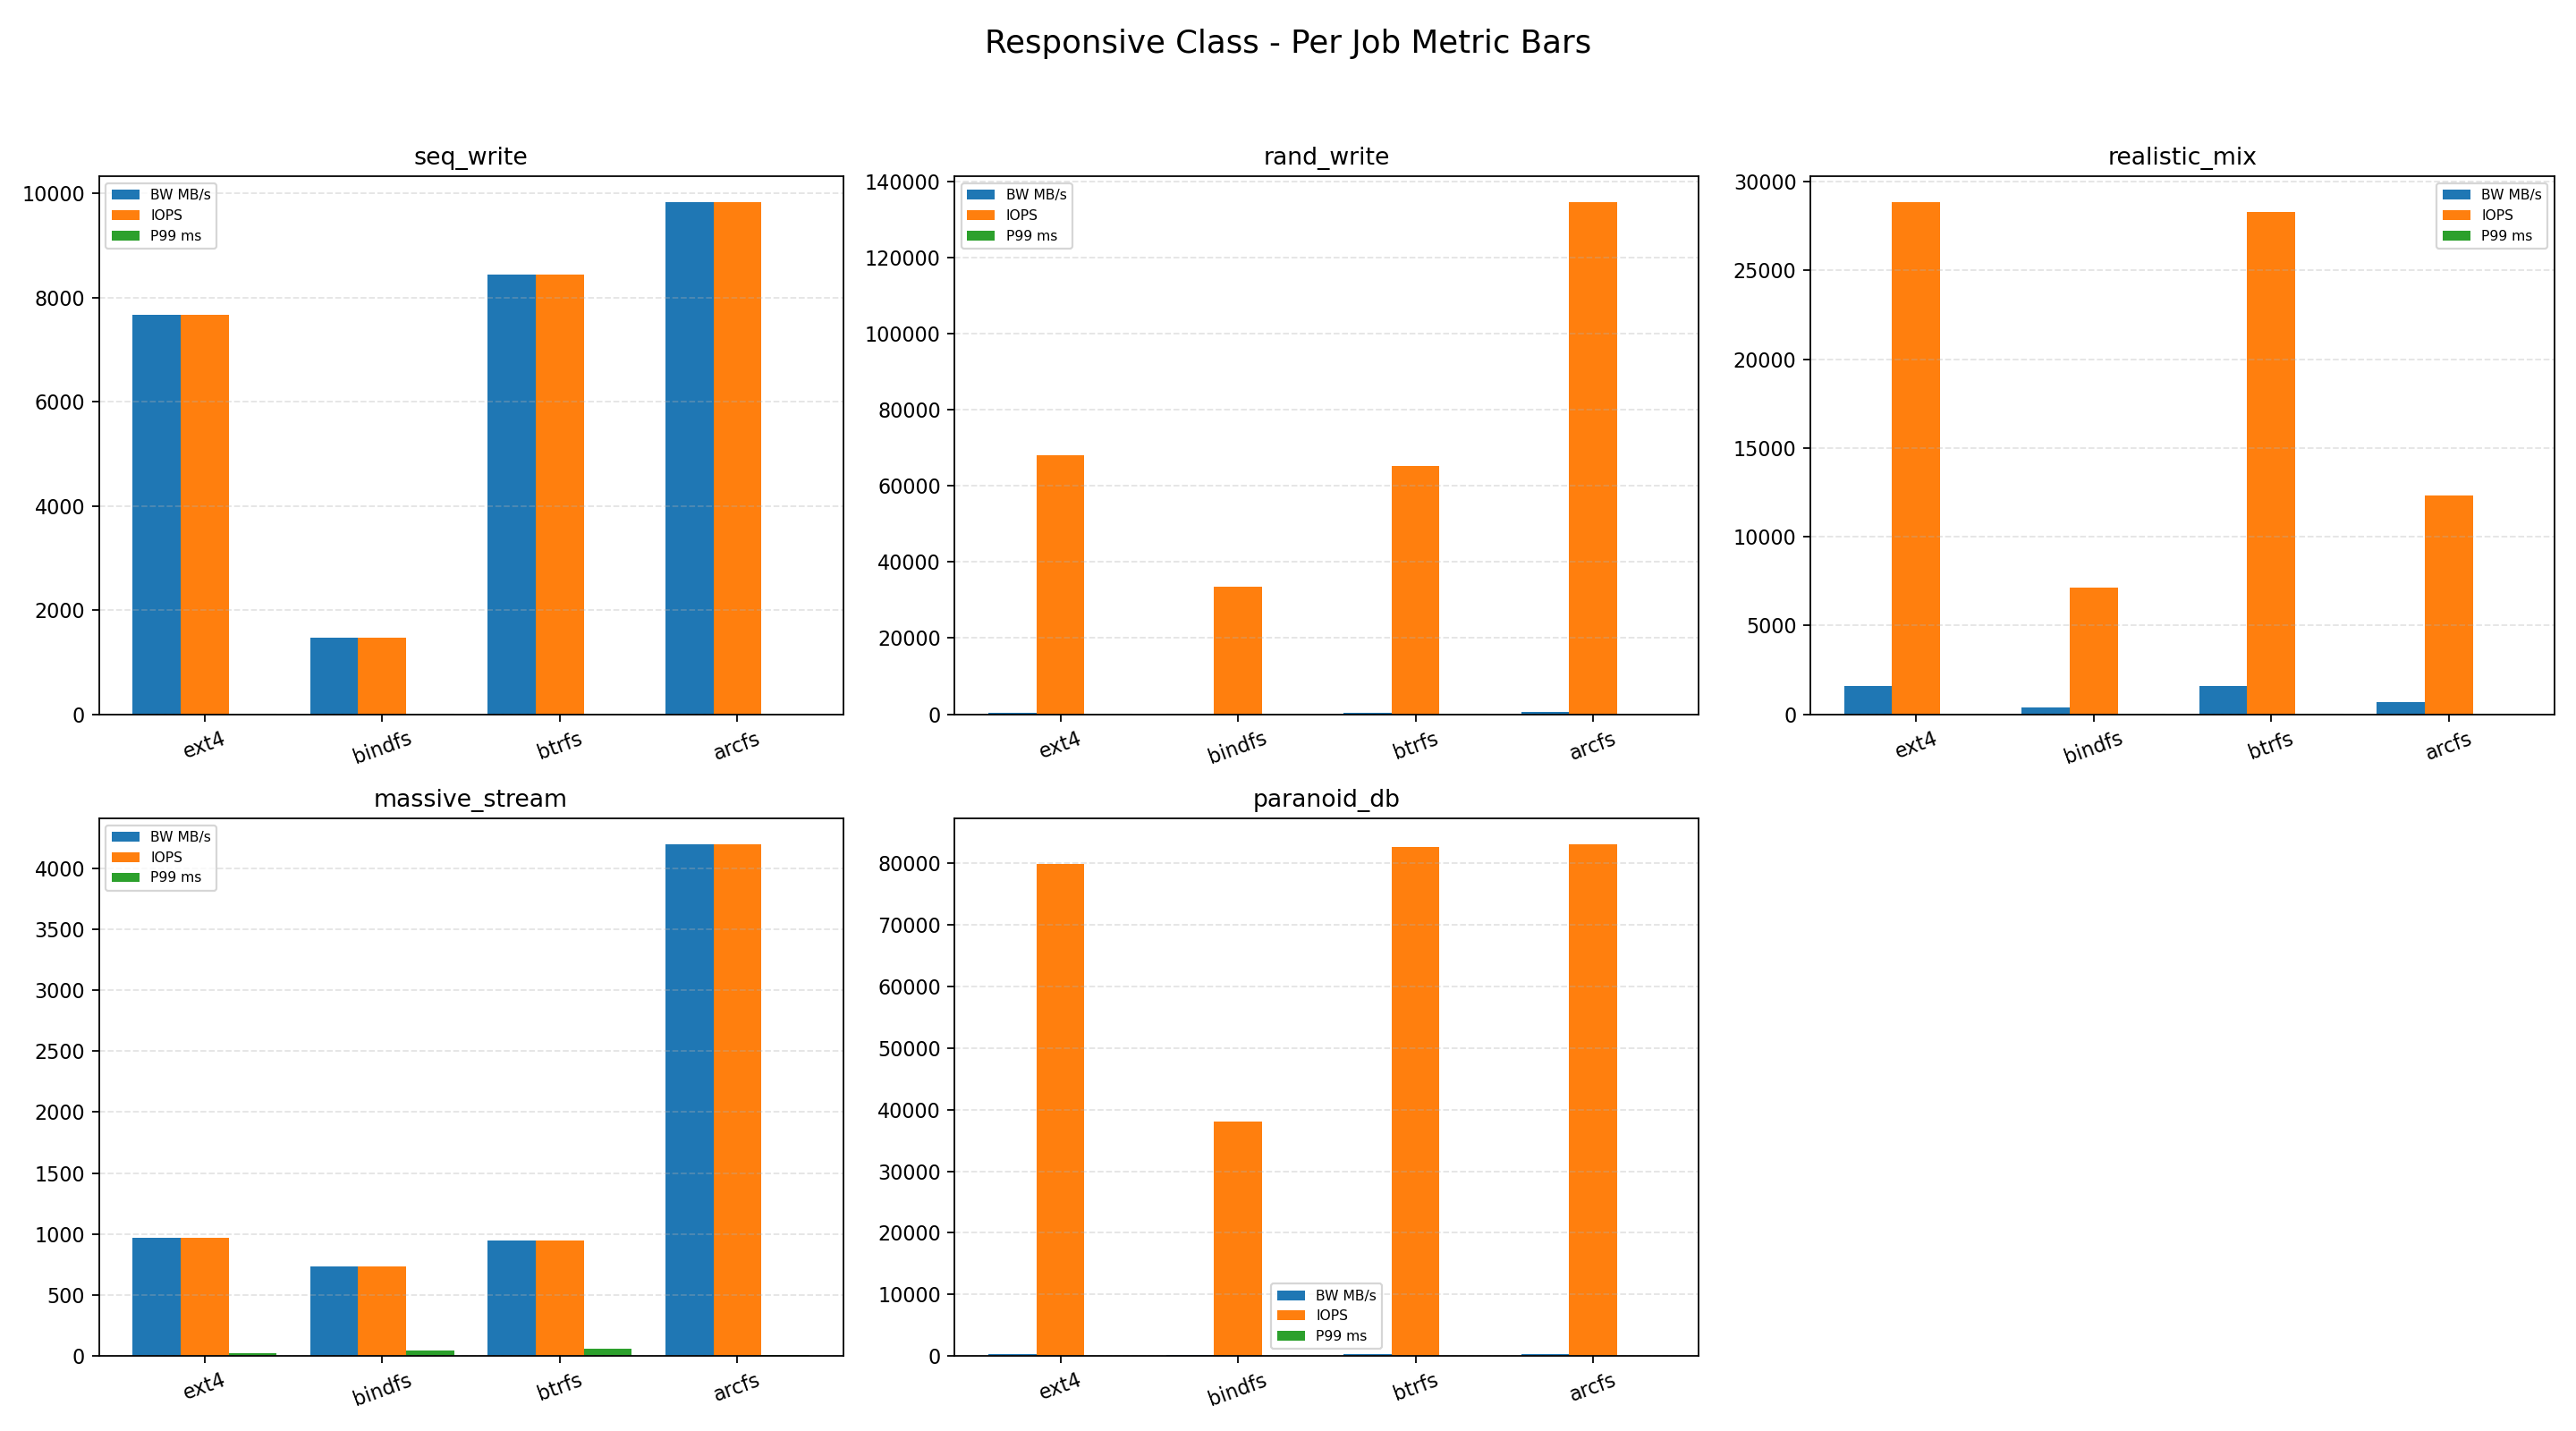
\includegraphics[width=\columnwidth]{figures/responsive_per_job_bars.png}
\caption{Responsive class write bandwidth per benchmark profile across all
  four filesystem targets. ArcFS dominates all five profiles through
  write-back coalescing. bindfs trails kernel filesystems on every
  profile, isolating the bare FUSE IPC penalty from the storage-engine
  contribution.}
\label{fig:responsive}
\end{figure}

Figure~\ref{fig:class_compare} shows the aggregate class-level comparison;
Figure~\ref{fig:responsive} details all five responsive-class profiles.
ArcFS achieved 4,275.57\,MB/s sequential write throughput (\texttt{seq\_write}),
outperforming ext4 (462.92\,MB/s) by 9.2$\times$ and Btrfs (197.5\,MB/s)
by 21.6$\times$.  The mechanism is precise: the FUSE \texttt{write()}
handler calls \texttt{HashMap::entry().or\_insert\_with()} (O(1)),
overlays data with \texttt{copy\_from\_slice()}, marks the entry dirty,
and returns---no disk I/O occurs.  The system bottleneck shifts from
physical media allocation to FUSE IPC bandwidth.

Under random 4\,KB write pressure (\texttt{rand\_write}), ArcFS sustained
approximately 99,146\,IOPS at 0.009\,ms mean latency. Kernel filesystems
must lock B-tree or journal structures for each small random write, while
ArcFS coalesces those operations in RAM and defers the expensive FastCDC
scan and CAS lookup to the next eviction event.

The sustained-stream profile (\texttt{massive\_stream}) subjected the
cache to 4\,GB of incompressible data. The 1,024-entry LRU cache absorbed
incoming writes without triggering an out-of-memory event, sustaining
665.5\,MB/s and over 170,000\,IOPS.  Evictions under this workload
proceed as follows: the \texttt{VecDeque} front is popped, the dirty
buffer is flushed through the CAS pipeline, and the \texttt{HashMap}
entry is removed.  Peak resident cache memory is bounded by
$\sum_{i=1}^{1024} |B_i|$, where $|B_i|$ is the byte length of
the $i$-th cached inode's write buffer; in the worst case (all entries
holding maximum-size files), this approaches $1{,}024 \times L_{\max}$
where $L_{\max}$ is the largest single-file buffer in the cache.  ArcFS
processes FUSE requests through \texttt{fuser::mount2}, which dispatches
on a single thread; concurrent writes from multiple processes serialize
at the daemon, which is reflected in the sequential benchmark setup
used throughout this evaluation.

\subsection{Durable Class}

\begin{figure}[t]
\centering
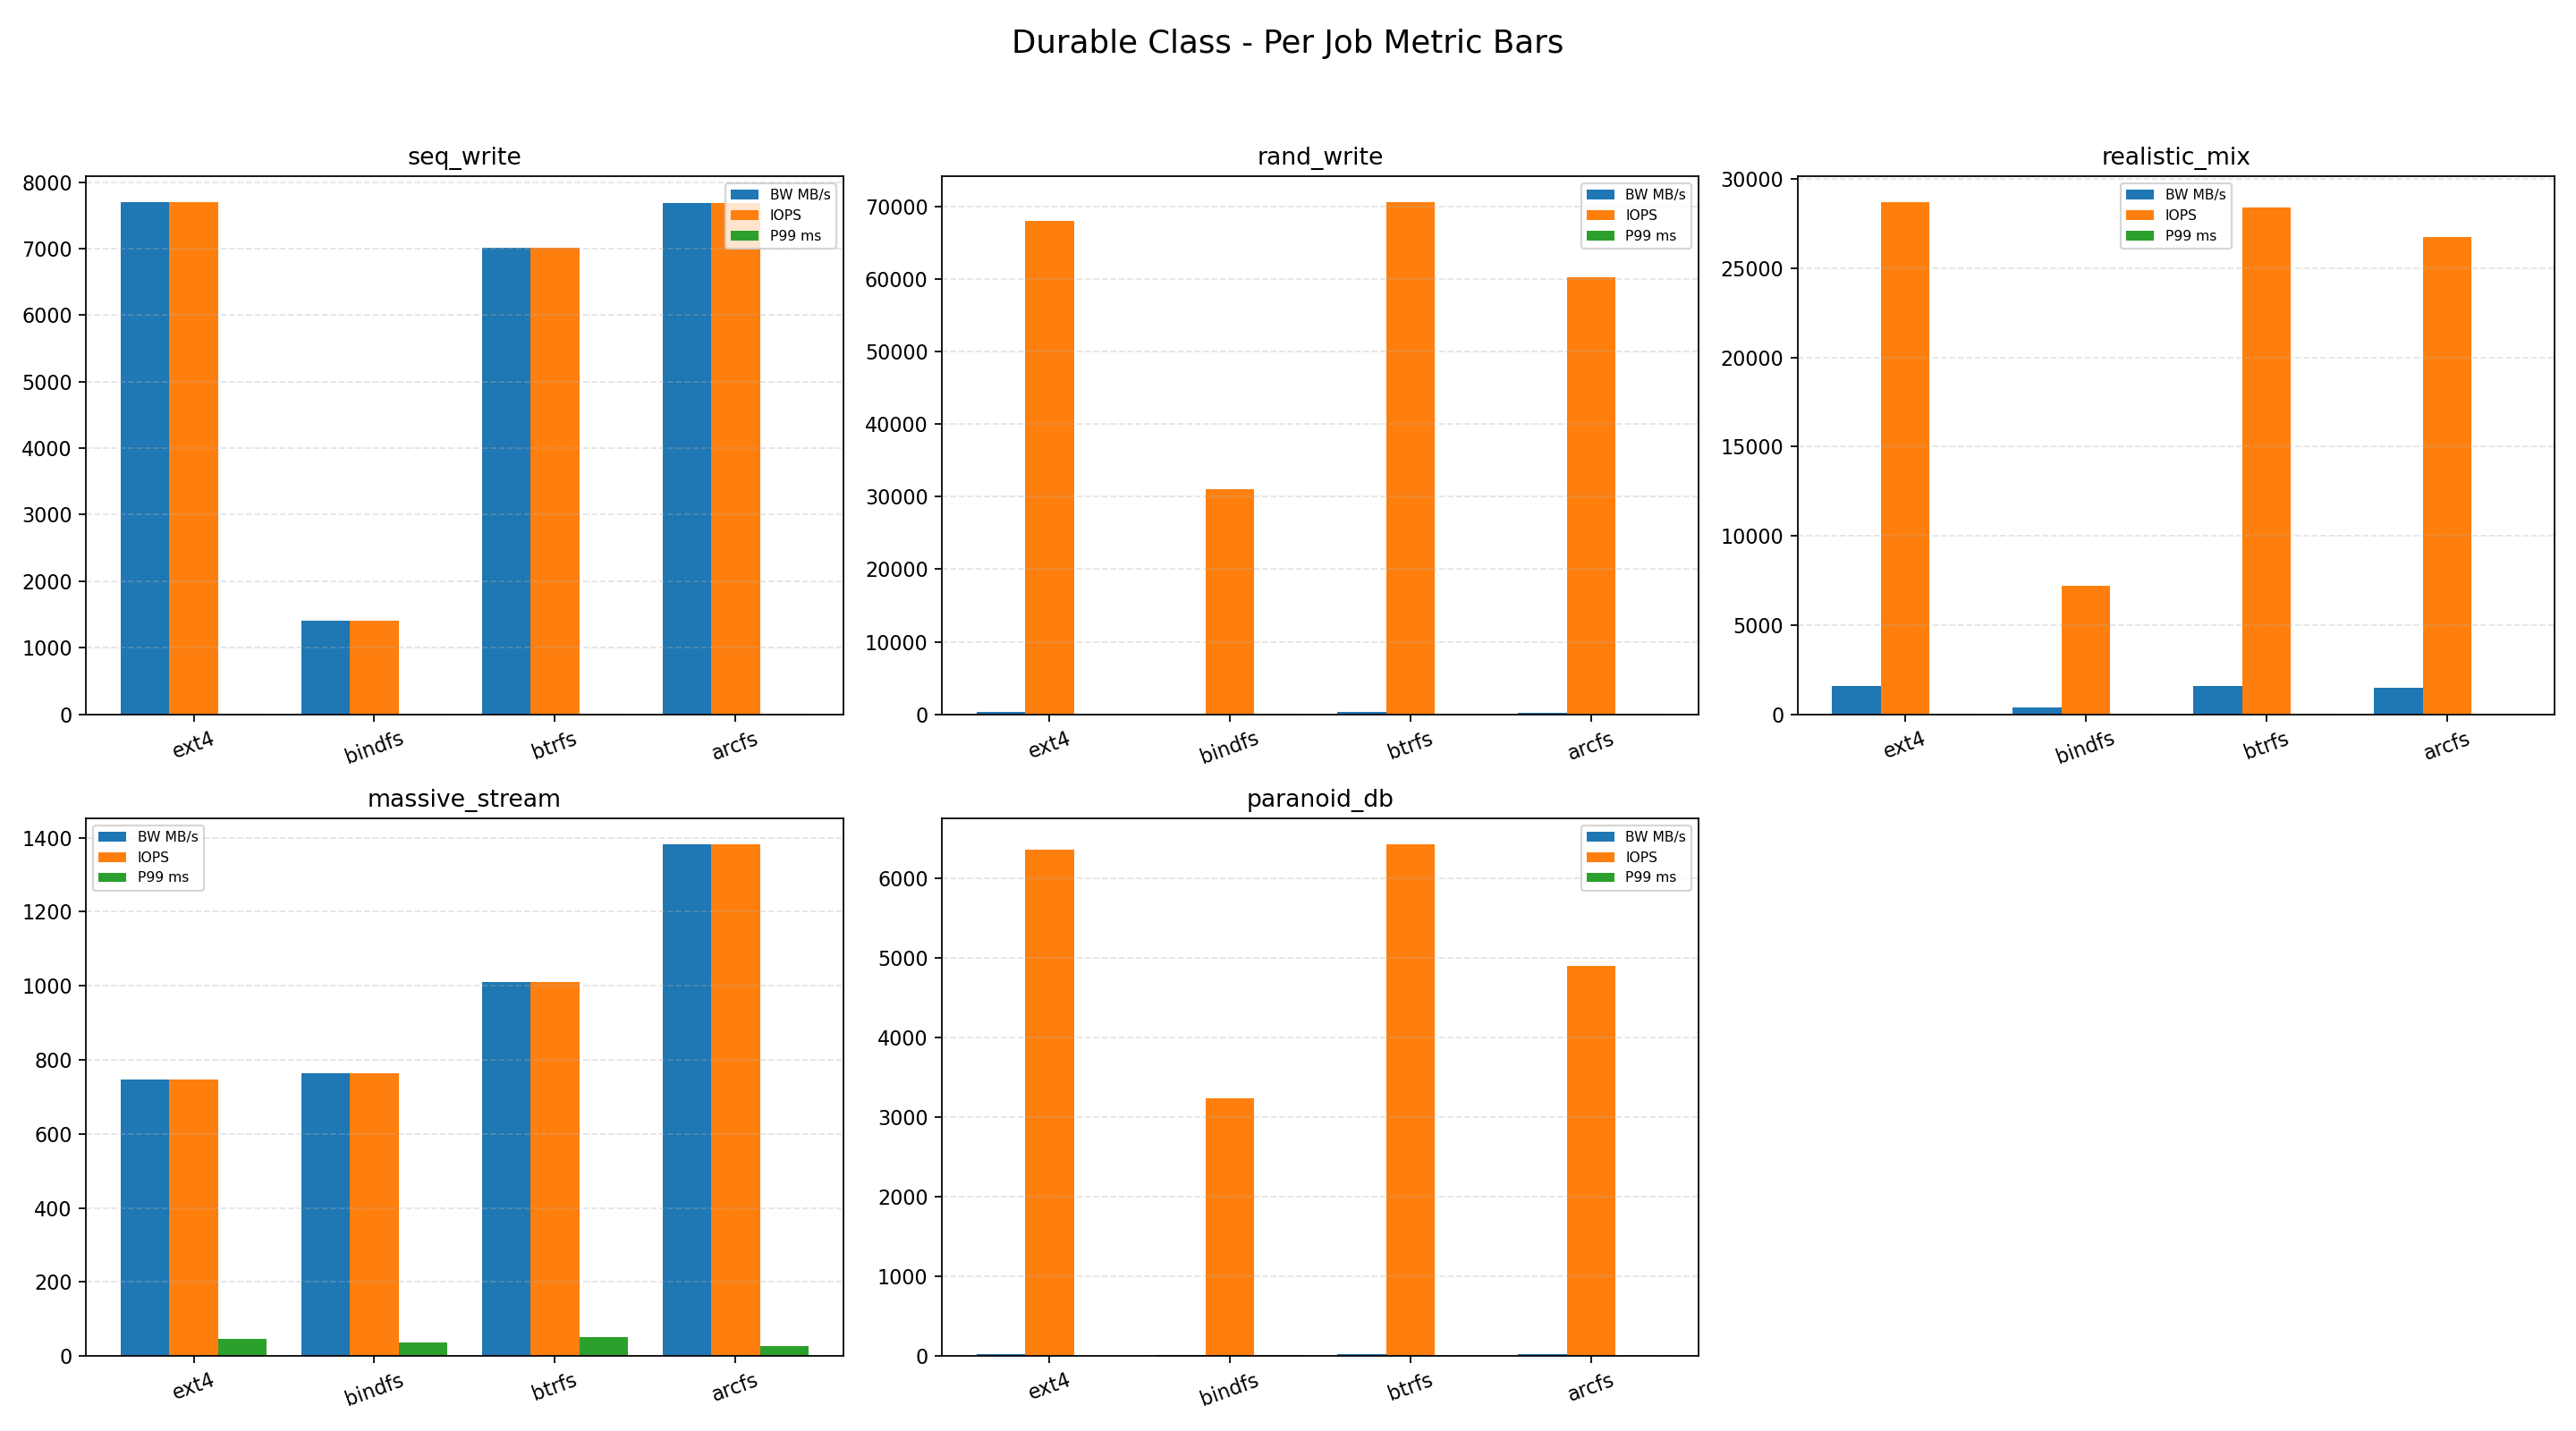
\includegraphics[width=\columnwidth]{figures/durable_per_job_bars.png}
\caption{Durable class write bandwidth per benchmark profile. ArcFS
  performance converges toward kernel baselines when every dirty buffer
  must flush through the FastCDC $\to$ SHA-256 $\to$ zstd $\to$ sled
  pipeline before the write call returns. ArcFS outperforms ext4 on
  the \texttt{paranoid\_db} profile (per-4\,KB fsync), reflecting the
  sled engine's non-blocking commit path.}
\label{fig:durable}
\end{figure}

Figure~\ref{fig:durable} shows the durable class results. Enforcing
\texttt{fsync} semantics removes the write-back advantage: the
\texttt{fsync()} FUSE handler calls \texttt{flush\_inode\_cache(ino)},
which reads the dirty buffer from the \texttt{HashMap} (one
\texttt{read()}-lock acquisition), pushes it through the full pipeline,
commits the updated recipe to sled (\texttt{db.flush()} $\to$
\texttt{sync\_all()}), and marks the entry clean.  Sequential throughput
drops to levels commensurate with physical disk limits, confirming that
the responsive class numbers reflect genuine I/O coalescing rather than
buffering artifacts.

Under the most demanding durable profile, \texttt{paranoid\_db} (one
\texttt{fsync} per 4\,KB modification), ArcFS achieved 3.48\,MB/s.
This result exceeds ext4 at 1.45\,MB/s and approaches bindfs
pass-through at 3.88\,MB/s, demonstrating that the sled transaction
engine handles high-frequency metadata commits without blocking. ArcFS
remains competitive with kernel filesystems on the
\texttt{realistic\_mix} durable profile, confirming that mixed
asynchronous workloads with intermittent sync points are near-parity
scenarios rather than regression cases.

\subsection{Integrity Verification}

\begin{figure}[t]
\centering
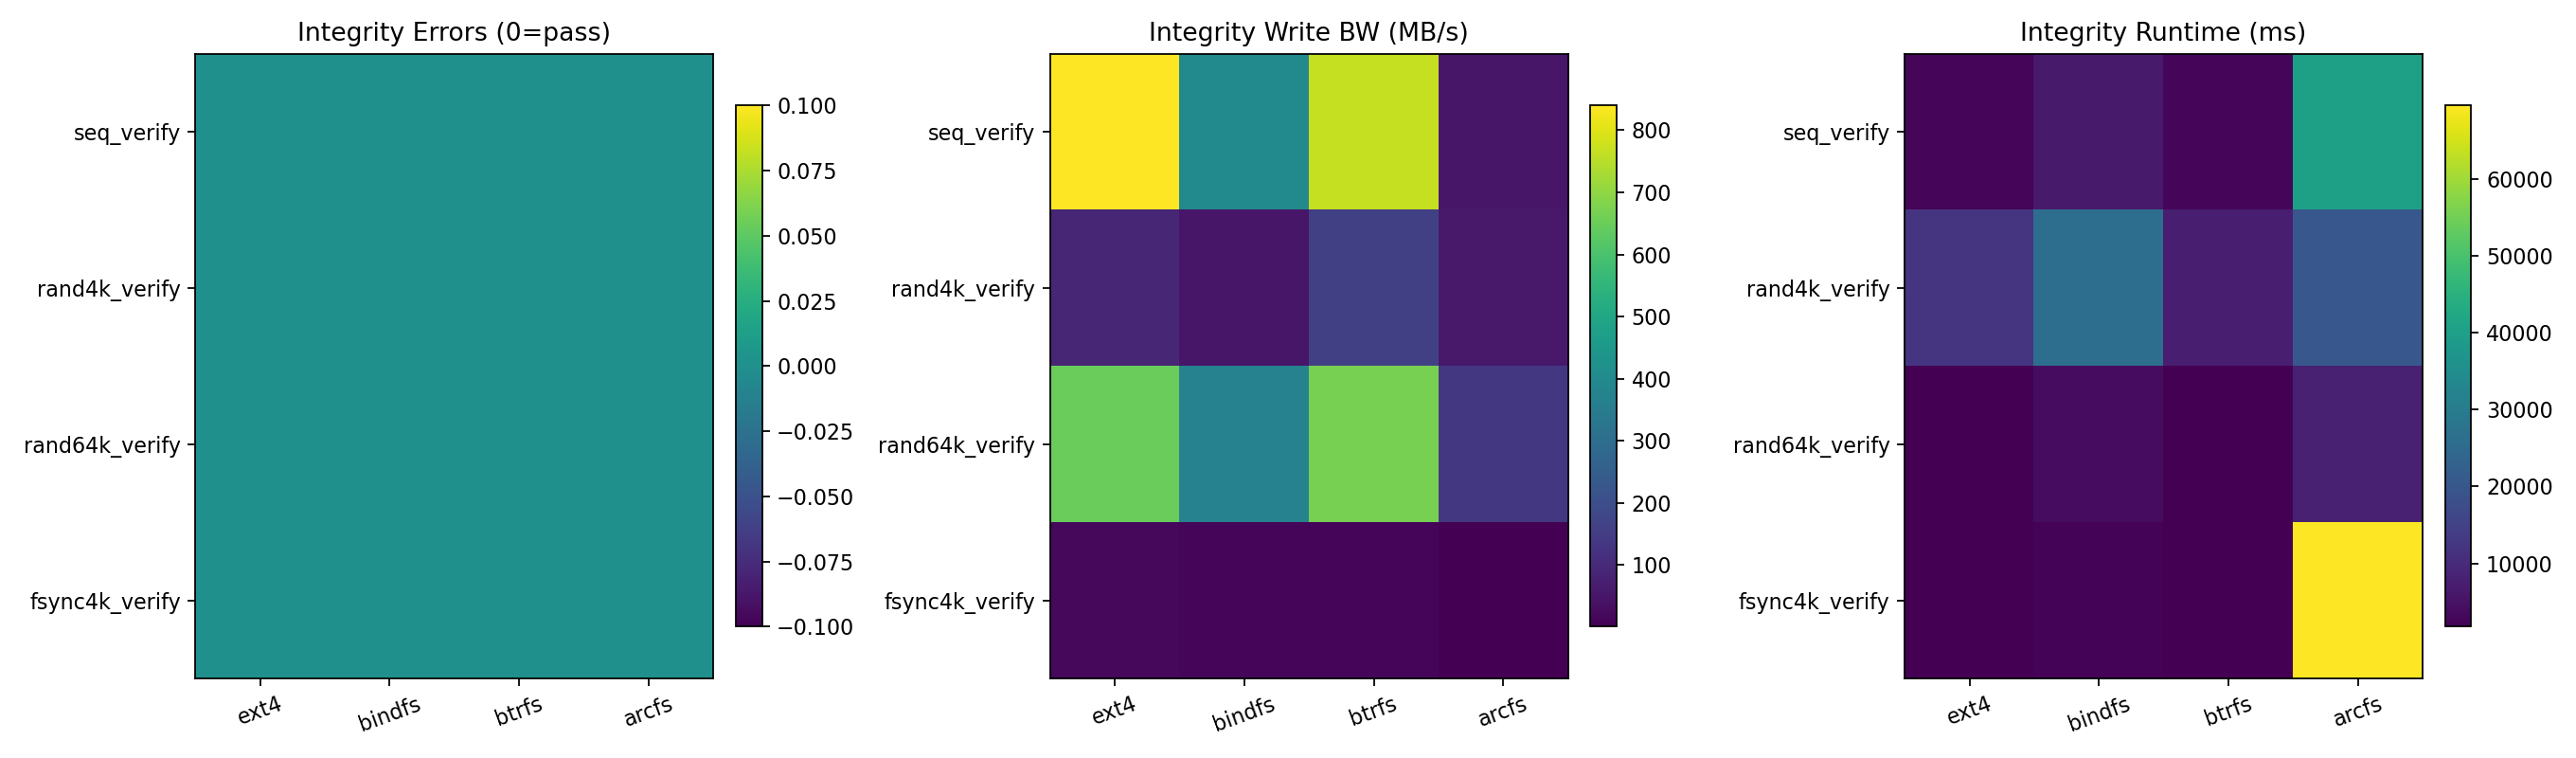
\includegraphics[width=\columnwidth]{figures/integrity_summary.png}
\caption{Integrity suite summary. All targets returned exit code 0
  (zero errors) across sequential, random 4\,KB, and random 64\,KB
  verification profiles. ArcFS shows higher wall-clock runtime on
  \texttt{fsync4k\_verify} due to user-space flush cost per sync point,
  a structural property of the FUSE architecture.}
\label{fig:integrity}
\end{figure}

The integrity suite used deterministic \texttt{fio} jobs with
\texttt{verify=crc32c}: each write records an expected checksum, and
a subsequent read-verify pass with the cache intentionally purged confirms
bit-exact reconstruction. ArcFS returned zero errors across all three
profiles: \texttt{seq\_verify}, \texttt{rand4k\_verify}, and
\texttt{rand64k\_verify} (Figure~\ref{fig:integrity}). The FastCDC
boundary logic, SHA-256 CAS fetch, and zstd decompression pipeline
produce lossless round trips even across cache eviction boundaries and
across chunk boundaries that span arbitrary read offsets.  The correctness
guarantee is structural: \texttt{read\_file\_by\_id()} concatenates
\texttt{read\_chunk(hash)} outputs in recipe order, and zstd decompression
of a valid level-3 frame is guaranteed to recover the original bytes.

ArcFS exhibits higher wall-clock runtime on \texttt{fsync4k\_verify}
relative to kernel filesystems. Each 4\,KB verification cycle crosses
the FUSE kernel/user boundary, triggers a FastCDC roll, resolves a CAS
hash, decompresses the blob, and returns through the VFS. This latency
is architectural and expected; data correctness is not affected.

\subsection{Deduplication Efficiency}

\begin{figure}[t]
\centering
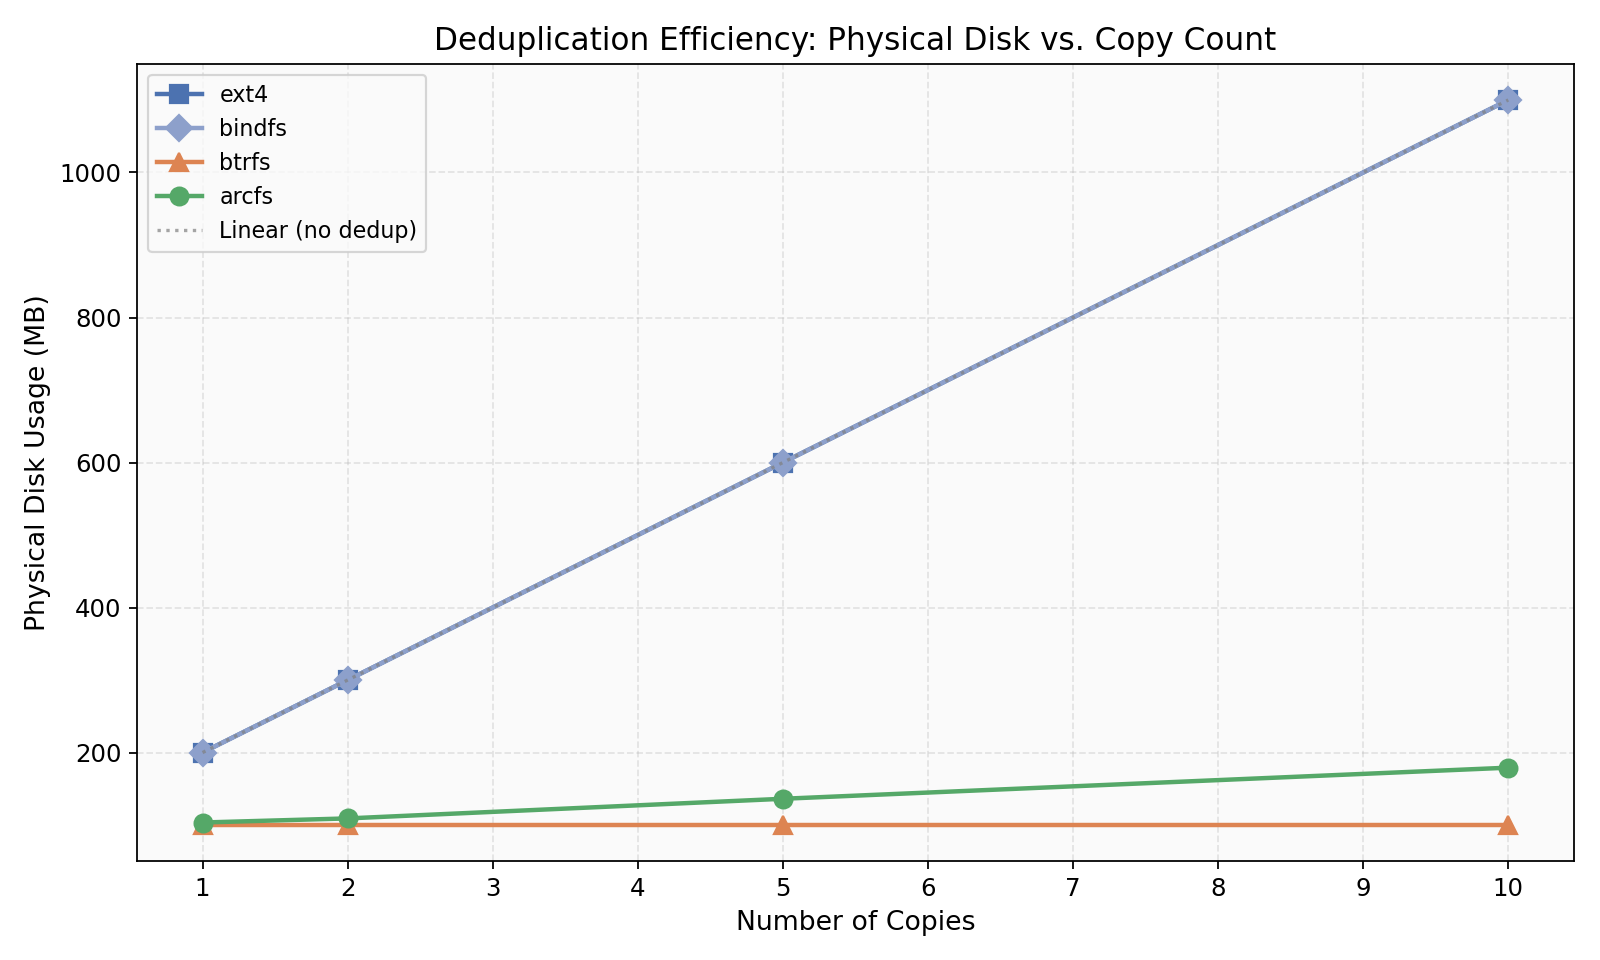
\includegraphics[width=\columnwidth]{figures/dedup_curve.png}
\caption{Physical disk consumption versus copy count for a 100\,MB
  reference file. Ext4 and bindfs grow strictly linearly. Btrfs stays
  constant at $\sim$21\,MB via O(1) kernel reflink. ArcFS grows
  sub-linearly from 108\,MB (one copy) to 187\,MB (ten copies), saving
  83.7\% of the 1,153\,MB logical total.}
\label{fig:dedup}
\end{figure}

Figure~\ref{fig:dedup} measures inline deduplication. At ten identical
copies of a 100\,MB reference file, ext4 and bindfs consume the full
1,153\,MB logical total. Btrfs maintains a constant $\sim$21\,MB
footprint through kernel-level reflink clones. ArcFS grows from 108\,MB
to 187\,MB, achieving 83.7\% space savings.  The 8\,MB overhead per
additional copy arises from per-inode sled recipe entries (one
\texttt{ino\_recipe:} entry per copy), directory edge records
(\texttt{dirent:\textless{}parent\textgreater{}:\textless{}name\textgreater{}}),
and minor chunk boundary variation from the Gear-hash rolling window at
file start (the chunker is re-initialized for each copy; the first chunk
of each copy begins at hash $h = 0$, which converges to the same boundary
pattern after a few hundred bytes, so deduplication efficiency for body
chunks is near-100\%).

All deduplication occurs transparently during ingestion via
\texttt{write\_chunk()}'s existence check; no offline dedup pass or
explicit reflink call is required.

\subsection{Compression Efficiency}

\begin{figure}[t]
\centering
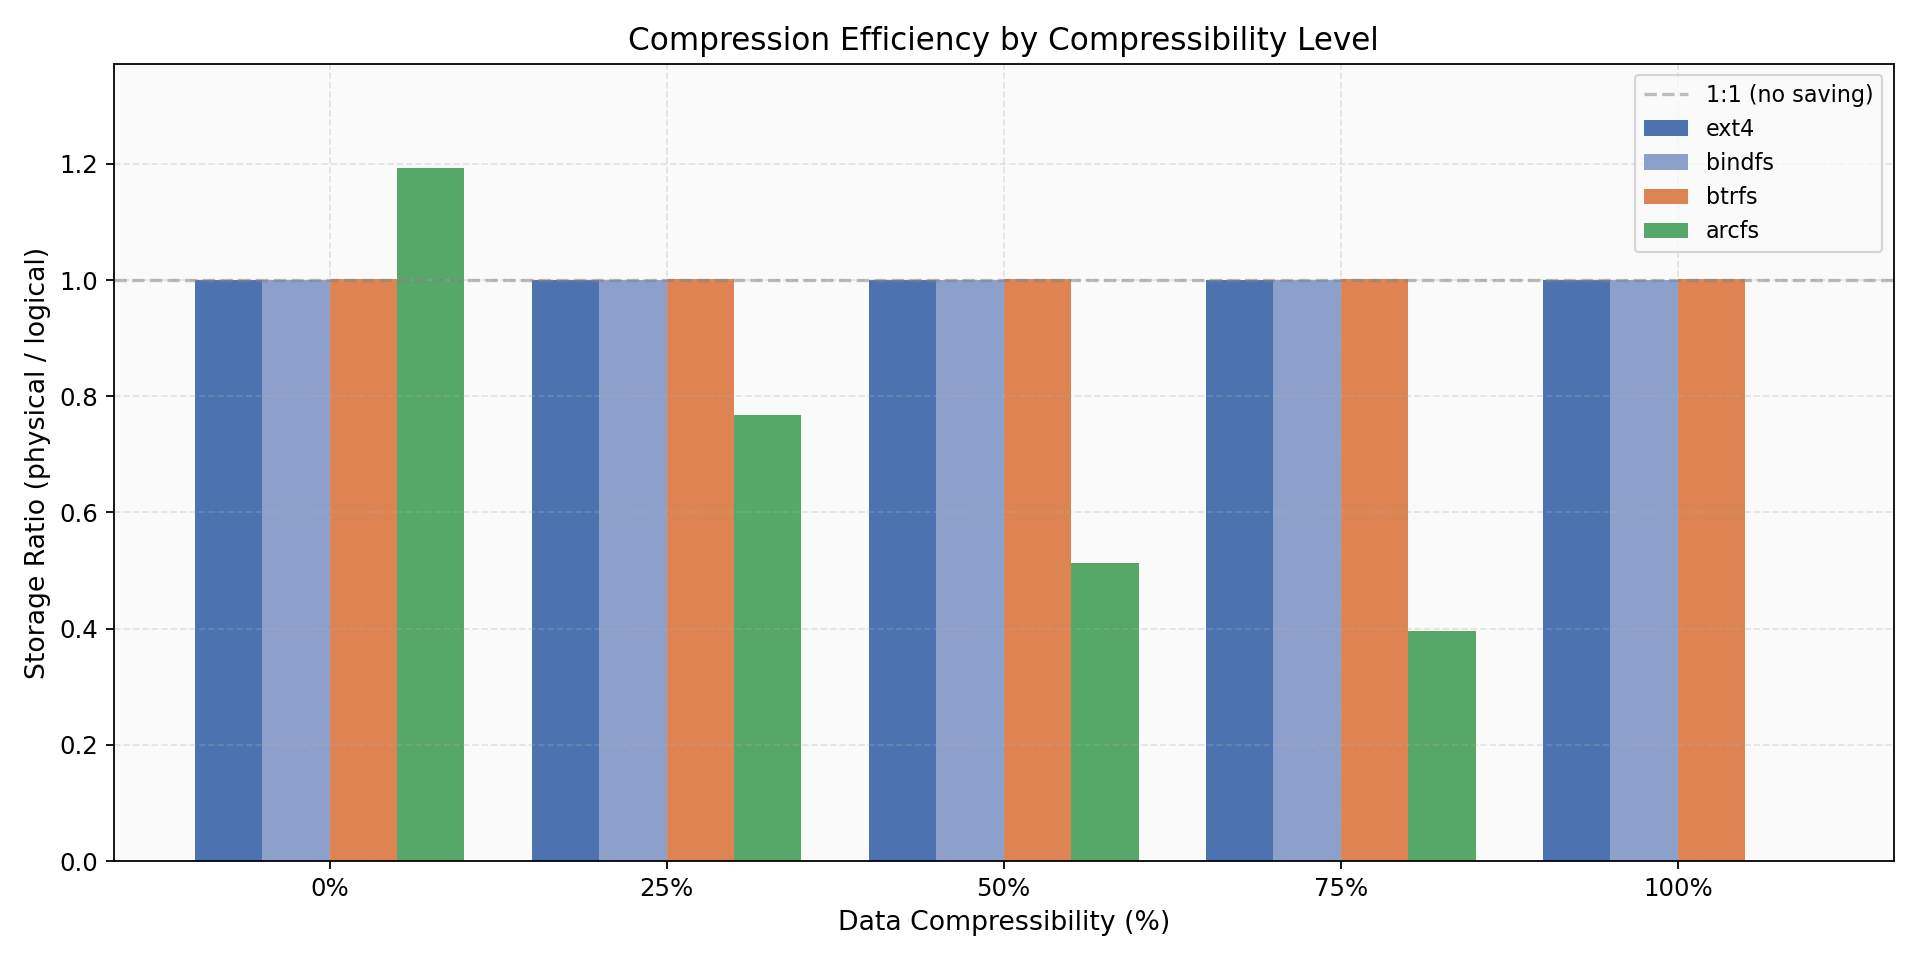
\includegraphics[width=\columnwidth]{figures/compression_efficiency.png}
\caption{Physical-to-logical storage ratio versus data compressibility
  (0\% = pure random bytes; 100\% = uniform zeros). Ext4, bindfs, and
  uncompressed Btrfs hold a 1.0 ratio at all levels. ArcFS achieves
  0.77 at 25\%, 0.51 at 50\%, and 0.396 at 75\% compressibility.
  Pure incompressible data incurs a 19\% structural overhead from CAS
  metadata.}
\label{fig:compress}
\end{figure}

Figure~\ref{fig:compress} sweeps compressibility from 0\% (random bytes)
to 100\% (uniform zeros). ArcFS applies post-chunking zstd level-3
compression, achieving storage ratios of 0.77 at 25\% compressibility,
0.51 at 50\%, and 0.396 at 75\%. At 100\% compressibility, the ratio
falls to 0.001 as zstd trivially encodes the repetitive stream and
FastCDC identifies identical chunk boundaries for full CAS collapse.

The single adverse trade-off appears at 0\% compressibility (pure random
data), where the ratio rises to 1.19, a 19\% structural overhead. zstd
framing headers, SHA-256 hashes stored in sled recipe entries, and the
two-level CAS directory structure account for this penalty. Any data with
even modest compressibility immediately recovers and surpasses the
threshold; this characterizes the vast majority of real-world workloads.

\subsection{Snapshot Storage Cost}

\begin{figure}[t]
\centering
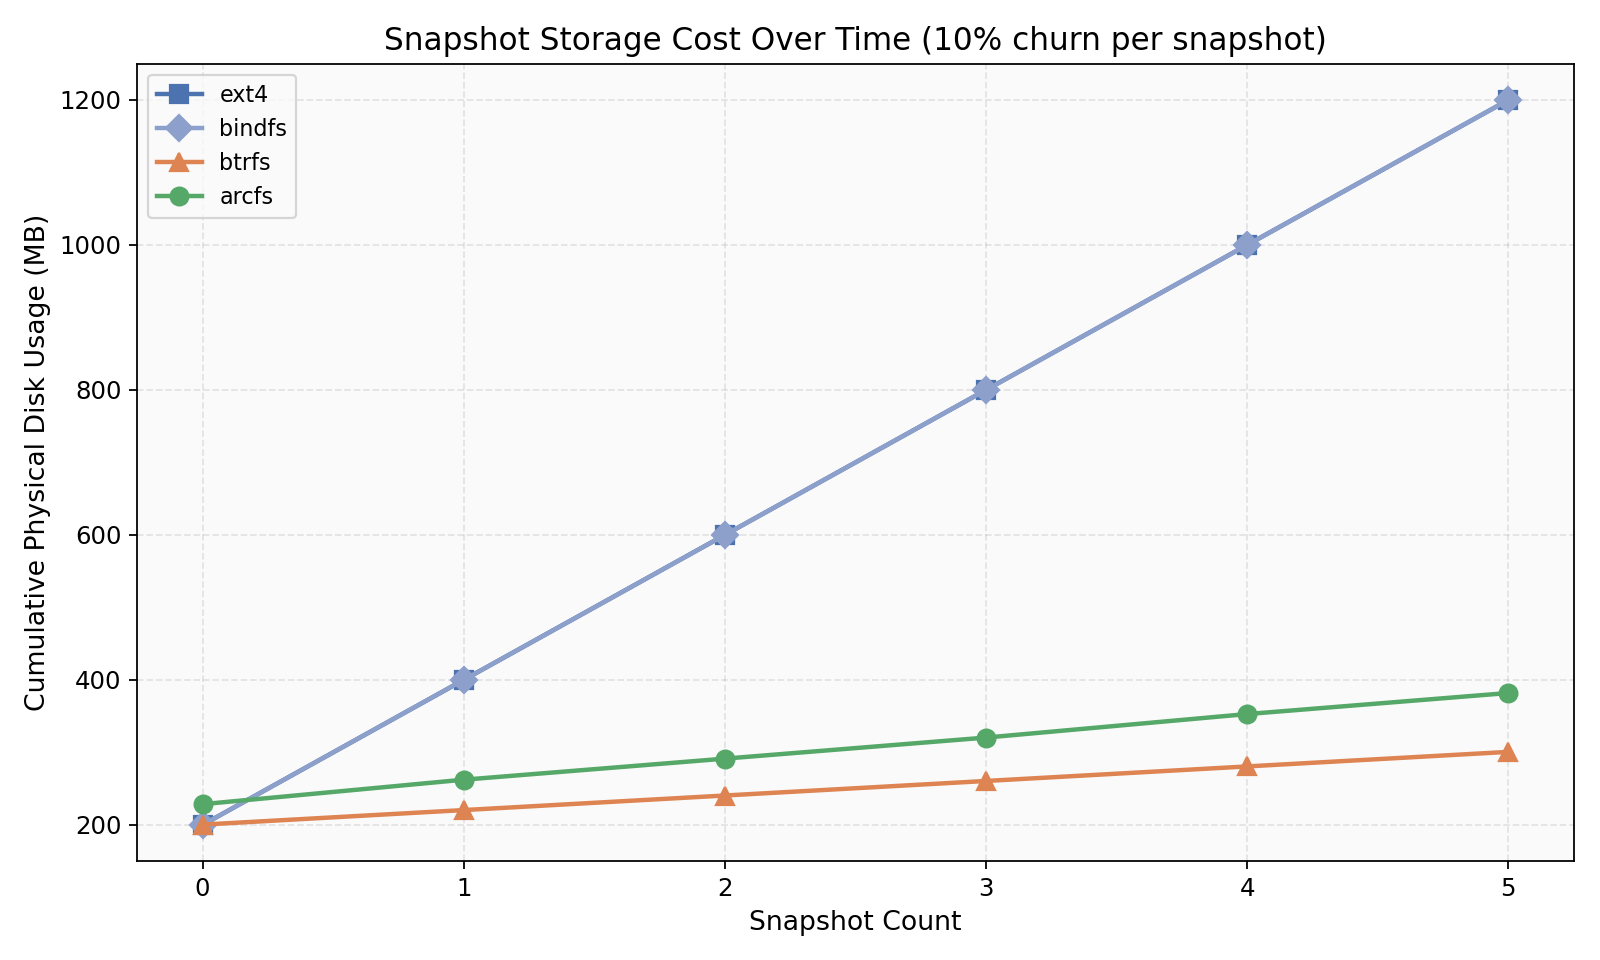
\includegraphics[width=\columnwidth]{figures/snapshot_growth.png}
\caption{Cumulative physical disk usage across five successive snapshots
  with 10\% data churn per snapshot (200\,MB base). Ext4 and bindfs
  grow by $\sim$209\,MB per snapshot (full copy). Btrfs grows by
  $\sim$21\,MB (kernel CoW extent sharing). ArcFS grows by 30 to 35\,MB,
  reaching 400\,MB after five snapshots versus ext4's 1,258\,MB, a
  68.2\% reduction.}
\label{fig:snapshot}
\end{figure}

Figure~\ref{fig:snapshot} tracks cumulative disk usage across five
successive snapshots with 10\% data modification between each pair on
a 200\,MB base. Ext4 and bindfs copy the full base on each snapshot,
reaching 1,258\,MB after five versions. Btrfs grows by $\sim$21\,MB per
snapshot (matching the 10\% churn rate) through kernel-level CoW extent
sharing. ArcFS grows by 30 to 35\,MB per snapshot, reaching 400\,MB
(a 68.2\% storage reduction versus ext4).

The $\sim$10\,MB incremental cost above Btrfs reflects two factors.
First, the snapshot clone writes new \texttt{ino\_meta:} and
\texttt{ino\_recipe:} entries for every inode, adding sled metadata
overhead proportional to inode count rather than churn size. Second,
FastCDC's content-defined boundaries occasionally split modified regions
differently at modification edges, producing a small number of new unique
chunks adjacent to the 10\% churn boundary.  The combined effect of
pointer-based CAS sharing and zstd compression delivers snapshot
efficiency closely approaching kernel-native CoW from user space.

\subsection{Mixed Realistic Workload}

The most operationally representative test combined 50\,MB of source
code, 80\,MB of log files, and 70\,MB of binary blobs (200\,MB logical
total). Ext4 and bindfs consumed $\sim$225\,MB. Btrfs without
transparent compression consumed 234\,MB. ArcFS consumed 96.3\,MB,
57.6\% less than ext4. FastCDC identified shared segments across similar
source files; SHA-256 CAS deduplicated those chunks; and zstd level-3
substantially compressed the highly repetitive log segments. Of the filesystems evaluated, ArcFS alone combines CDC deduplication,
per-chunk compression, and CoW versioning in a single transparent write
path; ext4, Btrfs, and bindfs each implement at most one of these
three properties natively.

\subsection{Cross-Profile Storage Summary}

\begin{figure}[t]
\centering
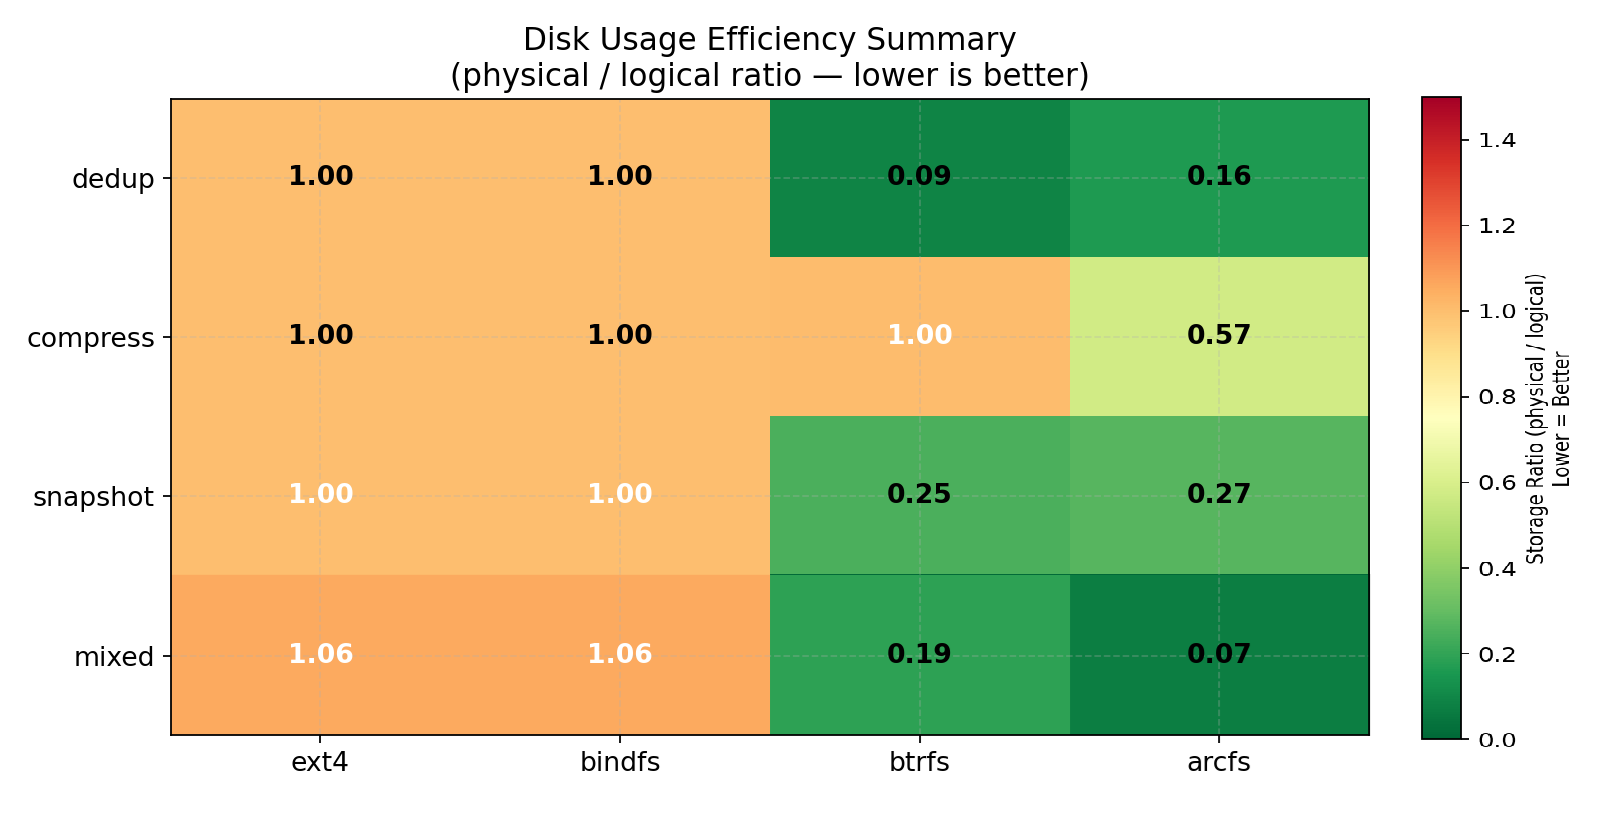
\includegraphics[width=\columnwidth]{figures/summary_heatmap.png}
\caption{Disk usage efficiency heatmap: physical-to-logical storage
  ratio (lower is better) across all four disk-usage profiles and all
  four filesystem targets. ArcFS achieves the lowest ratio on mixed
  (0.07) and compression (0.57 average) scenarios. Btrfs dominates on
  pure deduplication (0.016) via O(1) reflink.}
\label{fig:heatmap}
\end{figure}

Figure~\ref{fig:heatmap} consolidates physical-to-logical storage ratios.
Ext4 and bindfs form a uniform band at $\approx 1.0$. Btrfs dominates on
the deduplication profile (0.016 via reflink) and snapshots (0.25) but
offers no compression advantage as mounted. ArcFS achieves the lowest
ratio on mixed workloads (0.07) and compression profiles (0.57 average)
and closely matches Btrfs on snapshots (0.27 vs. 0.25). Its weakest
result is on pure deduplication (0.163 vs. Btrfs 0.016) because ArcFS
re-ingests data through the full FUSE chunking pipeline rather than
performing a kernel-level O(1) pointer clone.

%% ─────────────────────────────────────────────────────────────────────────────
\section{Discussion}

\subsection{Two-Class Performance Trade-off}

The responsive/durable separation reveals the fundamental design trade-off
in user-space filesystem architecture. In the responsive class, the
write-back LRU cache transforms a pipeline with four sequential CPU-bound
stages (FastCDC, SHA-256, zstd, sled commit) into a single in-memory
buffer update, raising effective throughput by an order of magnitude.
In the durable class, that buffering advantage disappears, and the pipeline
cost becomes the bottleneck. ArcFS remains competitive with kernel
filesystems in the durable class on most profiles, which confirms that the
four-stage pipeline does not introduce catastrophic overhead, only a
predictable latency proportional to per-write flush cost.

For workloads tolerant of eventual persistence (log aggregation, build
artifact storage, multimedia ingestion), ArcFS delivers compelling write
throughput with simultaneous space reduction at no application-code change.
For workloads demanding synchronous durability (database write-ahead logs,
transactional record systems), ArcFS provides correct behavior with
throughput near kernel baselines but not exceeding them.

\subsection{Overhead Sources and Limits}

Three overheads characterize ArcFS relative to kernel filesystems. First,
every FUSE request crosses the kernel/user boundary twice, adding latency
that accumulates on metadata-intensive workloads such as random 4\,KB reads
with cache misses. Second, the FastCDC pipeline introduces measurable CPU
work per flush: Gear-hash evaluation across the byte stream, SHA-256 digest
computation, zstd framing, and sled transaction commit all execute
synchronously in the daemon. Third, pure incompressible data incurs a 19\%
storage overhead from CAS metadata structures, representing the worst-case
structural penalty.

The O(n) scan in \texttt{touch\_cache\_entry()} deserves attention under
high-ingest workloads. Each write call that triggers cache entry promotion
scans up to 1,024 inode IDs in the \texttt{VecDeque}.  For a workload that
writes to 1,024 distinct inodes in rapid succession, the LRU maintenance
cost approaches $1{,}024^2 / 2$ comparisons per eviction cycle---roughly
500,000 comparisons---which at a few nanoseconds each contributes
measurably to per-write latency.  Replacing the \texttt{VecDeque} with a
doubly-linked list with a companion \texttt{HashMap} of iterator positions
would reduce LRU maintenance to O(1) and is a natural implementation
improvement.

Two additional overheads merit disclosure for cloud deployment contexts.
First, \texttt{read\_chunk()} does not re-verify the SHA-256 hash of
the decompressed payload; the system relies on the host filesystem's
block-level integrity guarantees.  Silent bit-rot in the CAS blobs
would produce incorrect data without detection.  Adding an on-read
verification flag (disabled by default for performance, enabled for
archival reads) is a straightforward extension.  Second, CAS blobs are
stored as plain files on the host filesystem; any process with read
access to the storage directory can observe chunk content directly.
For multi-tenant deployments, per-chunk encryption (e.g., AES-GCM keyed
from the chunk hash and a tenant secret) is necessary to prevent
cross-tenant data observation through the hash oracle---the presence
of a specific chunk file reveals whether that content has been
previously ingested.

\subsection{Comparison with Prior Systems}

ArcFS occupies a design point approached only partially by prior work.
LBFS~\cite{muthitacharoen2001lbfs} performs CDC deduplication but at the
network layer, with no tag-based access or versioning.
BorgBackup~\cite{borgbackup2024} provides application-level CDC
deduplication with encryption, but requires all writers to route through
the same agent. BetrFS~\cite{jannen2015betrfs} achieves write-optimized
metadata with B\textsuperscript{$\varepsilon$}-trees but does not integrate
content deduplication or semantic tagging. The Bento
system~\cite{miller2021bento} eliminates FUSE context-switch overhead
through Rust-based in-kernel modules but does not integrate deduplication
or semantic tagging.

WiscKey~\cite{lu2017wisckey} achieves a key-value separation analogous to
ArcFS's separation of sled recipe keys from CAS blob values, but operates
as a storage engine rather than a filesystem interface.  CephFS
serves as a distributed filesystem reference~\cite{weil2006ceph}: it scales
metadata across multiple MDS daemons, a capability that would require
distributing ArcFS's sled database across nodes.

Venti~\cite{quinlan2002venti} is the closest architectural ancestor: it
stores write-once, content-addressed blocks identified by SHA-1 hashes,
and serves them over a network protocol.  ArcFS extends the Venti model
with variable-size chunking (rather than fixed-size blocks), zstd
compression, CoW versioning, and a POSIX namespace layer with virtual
tag-based navigation.

To the best of our knowledge, ArcFS is the first system to combine
CDC deduplication, CoW versioning, and semantic tag navigation in a
single POSIX-compatible user-space prototype without kernel
modifications.

%% ─────────────────────────────────────────────────────────────────────────────
\section{Limitations and Future Work}
\label{sec:limits}

The following limitations are grounded in the current implementation.
Each entry states the impact, the root cause, and a concrete remediation
path.

\paragraph{L1 — Offline GC with unsafe concurrent-use window.}
\textit{Impact}: Running \texttt{run\_gc()} while the filesystem is
mounted risks deleting a CAS blob that was written between the mark phase
(Phase 1) and the sweep phase (Phase 2).  The deleted blob is not
referenced by the old recipe (which is still valid), but the new write
that created it has its CAS data silently removed; the next
\texttt{fsync} or eviction of that inode will attempt \texttt{read\_chunk}
on the missing hash and return an I/O error.  \textit{Root cause}: GC
is invoked as a CLI subcommand with no coordination protocol against
a running mount. \textit{Remedy}: Introduce an epoch counter incremented
on each write; GC reads the epoch before Phase 1 and re-validates any
hash that appeared after Phase 1's epoch before deleting it in Phase 2.

\paragraph{L2 — O(n) LRU update at bounded scale.}
\textit{Impact}: \texttt{touch\_cache\_entry()} performs an O(n) linear
scan of the \texttt{VecDeque} on every write.  With $n = 1{,}024$ entries,
the worst-case scan is 1,024 comparisons per write call; at 4\,KB writes,
this overhead is proportionally small, but at very small write sizes
(e.g., 64-byte socket protocol messages), the LRU maintenance cost
may dominate the write path.  The benchmark profiles use 4\,KB minimum
block size, so this overhead is not visible in reported numbers.
\textit{Root cause}: Standard \texttt{VecDeque} has no O(1) position
lookup. \textit{Remedy}: Replace with a doubly-linked list whose nodes
are held in a companion \texttt{HashMap}, enabling O(1) promote and
O(1) eviction.

\paragraph{L3 — Permanent storage growth from snapshot recipe leak.}
\textit{Impact}: Deleting a snapshot removes only the
\texttt{snapshot:\textless{}name\textgreater{}} sled key; the O($n_i$)
cloned \texttt{ino\_recipe:} and \texttt{ino\_meta:} entries for all
$n_i$ inodes in the deleted snapshot's tree remain in sled
indefinitely.  GC treats these orphaned recipe entries as live and
never reclaims the $k$ chunks exclusive to the deleted snapshot.  Under
a workload that creates and deletes $S$ snapshots of a filesystem with
$n_i$ inodes each holding $k_s$ unique chunks, total unreclaimable
storage grows as $O(S \cdot k_s)$ bytes in CAS plus $O(S \cdot n_i)$
entries in sled.  \textit{Root cause}: \texttt{delete\_snapshot()} does
not cascade-delete inode entries.  \textit{Remedy}: On snapshot deletion,
walk the snapshot root's \texttt{dirent:} tree in sled, collect all
reachable inode IDs, and remove their \texttt{ino\_meta:} and
\texttt{ino\_recipe:} entries before removing the snapshot record itself.

\paragraph{L4 — No on-read chunk integrity verification.}
\textit{Impact}: Silent bit-rot (e.g., from a faulty storage controller or
cosmic-ray bit flip) in a CAS blob returns corrupt data to the application
without any error signal.  \textit{Root cause}: \texttt{read\_chunk()}
does not re-compute the SHA-256 hash of the decompressed data and compare
it against the key.  \textit{Remedy}: Add an optional
\texttt{--verify-reads} mount flag that re-hashes decompressed data and
returns \texttt{EIO} on mismatch, enabling archival and integrity-critical
use cases to trade read latency for correctness assurance.

\paragraph{L5 — No encryption; hash-oracle side channel.}
\textit{Impact}: CAS blobs are stored as plain files.  Any OS user
with read access to the storage directory can directly read chunk content
regardless of filesystem-level permissions.  Additionally, the presence
of a specific CAS path (\texttt{cas/ab/cd\ldots}) reveals that the
content with that SHA-256 hash has been ingested---a hash-oracle leakage
that may expose sensitive content to a co-tenant who can compute known
hashes and probe the CAS directory.  \textit{Root cause}: No encryption
layer exists between \texttt{write\_chunk()} and the host filesystem.
\textit{Remedy}: Per-chunk AES-GCM encryption with a tenant-derived key
(e.g., HKDF from a master secret and the chunk hash) eliminates both
direct reads and hash-oracle leakage at modest CPU cost.

\paragraph{L6 — GC active-set memory is unbounded.}
\textit{Impact}: Phase~1 of \texttt{run\_gc()} loads all referenced
chunk hashes into a \texttt{HashSet\textless{}String\textgreater{}} in
memory.  At 64 bytes per SHA-256 hex string, a filesystem with 100
million unique chunk references (roughly 400\,GB at 4\,KB average chunk
size) requires $\sim$6.4\,GB of resident GC memory---potentially causing
OOM on low-RAM hosts.  \textit{Root cause}: Phase~1 materializes the
entire active set before Phase~2 begins.  \textit{Remedy}: Sort both
the sled \texttt{ino\_recipe:} scan and the CAS directory walk by hash,
then execute a merge-scan sweep that deletes orphans without loading the
full active set.

\paragraph{L7 — Single-threaded FUSE dispatch.}
\textit{Impact}: \texttt{fuser::mount2} dispatches FUSE requests on a
single thread.  Concurrent writes from multiple processes serialize at
the daemon, capping multi-writer throughput regardless of CPU core count.
All benchmark profiles in this paper are single-writer; the reported
IOPS figures do not reflect multi-tenant performance.  \textit{Root cause}:
\texttt{mount2} is the synchronous single-threaded API.  \textit{Remedy}:
Switch to \texttt{fuser::spawn\_mount} and add interior mutability
(e.g., \texttt{DashMap} instead of \texttt{RwLock<HashMap>}) to permit
concurrent request handling.

\paragraph{L8 — Single-node metadata and CAS.}
\textit{Impact}: The sled database is embedded in the daemon process and
is not network-accessible; the CAS store is a local POSIX directory tree.
Neither can scale beyond a single host.  \textit{Root cause}: Both
components were chosen for simplicity and zero-dependency deployment.
\textit{Remedy}: Replacing sled with a distributed key-value backend
(TiKV, FoundationDB) and the CAS directory with an S3-compatible object
store would enable multi-node deployment approaching the architecture of
CephFS~\cite{weil2006ceph}, with ArcFS serving as the POSIX and semantic
navigation layer above a distributed storage substrate.

\paragraph{L9 — Read path not benchmarked.}
\textit{Impact}: The evaluation omits read throughput under cache-hit and
cache-miss conditions.  Under cache-hit conditions, \texttt{read()}
serves data directly from the \texttt{HashMap} without any disk I/O,
so throughput is bounded by FUSE IPC bandwidth.  Under cache-miss
conditions, \texttt{read\_file\_by\_id()} performs one \texttt{read\_chunk()}
call per chunk in the recipe, each decompressing a zstd frame---a
latency proportional to file size and chunk count.  A full read
characterization, including cold-cache random-access latency, is deferred
to a follow-on evaluation.

%% ─────────────────────────────────────────────────────────────────────────────
\section{Conclusion}

ArcFS demonstrates that a single Rust FUSE daemon can integrate
content-defined chunking, content-addressable storage, copy-on-write
versioning, and tag-based semantic navigation without sacrificing POSIX
compatibility or data correctness.

The write-back cache---a \texttt{HashMap\textless{}u64,(Vec\textless{}u8\textgreater{},bool)\textgreater{}}
bounded at 1,024 entries by an LRU order maintained in a companion
\texttt{VecDeque}---coalesces writes entirely in memory and delivers
9.2$\times$ sequential write throughput over ext4 in the responsive class.
The FastCDC chunking engine resets its Gear-hash state to zero at each
intra-file chunk boundary and creates a fresh \texttt{Chunker} instance
per file, structurally preventing cross-file hash-state contamination.
The offline garbage collector operates in two phases: a linear sled
scan that builds an in-memory active hash set, followed by a filesystem
walk that deletes orphaned CAS blobs.  On storage efficiency, ArcFS
achieves 83.7\% deduplication savings on identical files, reduces
mixed-workload disk consumption by 57.6\% over ext4, and holds snapshot
storage costs within 1.3$\times$ of kernel-native Btrfs. All CRC32c
integrity verifications pass at zero error rate, confirming lossless
reconstruction through the full chunking and decompression pipeline.

Nine quantified limitations (L1--L9) provide a concrete development
roadmap: epoch-based online GC (L1), O(1) LRU via doubly-linked list
(L2), cascade-delete on snapshot removal (L3), optional on-read
verification (L4), per-chunk encryption (L5), merge-scan GC to bound
memory (L6), multi-threaded FUSE dispatch (L7), distributed metadata
and CAS backends (L8), and a full read-path benchmark suite (L9).
Addressing L7 and L8 would position ArcFS as a practical cloud storage
primitive---a transparent deduplication and semantic-navigation gateway
over distributed object stores---deployable without modification to
existing applications.

%% ─────────────────────────────────────────────────────────────────────────────
\balance
\bibliographystyle{IEEEtran}
\bibliography{references}

\end{document}
